\chapter{椭圆方程}
\label{chap:elliptic-equations}

一块金属板的边缘保持固定温度，板内某些地方持续发热。足够久之后，温度不再变化。板上每一点的温度是多少？这个数不能只看这一点附近：边缘上任何一段的温度升高，源项在任何一处的增强，都会让板内处处的温度发生变化。平衡场的每个值都同时取决于整个区域的数据。

这种“牵一发而动全身”的结构决定了椭圆方程的提法和做法。它没有时间方向，不能从一个初始时刻往后推，只能在整个区域上一次解出来。数据必须放在边界上，而且边界条件的类型决定了问题是否可解，也决定了解是否唯一。

能写出解的情形只占少数，但它们把结构摆得最清楚。区间上积分两次，就能看到积分常数怎样被边界条件吃掉；Green函数告诉我们一处的点源在别处产生多大的响应；特征函数把求解变成逐个模式的除法，还会暴露零特征值这个危险的情形。这些计算都要求解足够光滑，而系数有间断、源项很粗糙时，经典意义下的解根本不存在。

于是要换一种提法：不再逐点要求方程成立，而是要求方程经过所有测试函数检验后成立。这样得到的弱形式把二阶方程变成一阶导数的积分关系，边界条件也分成了写进空间和写进积分两种。Lax--Milgram定理随后给出存在、唯一和连续依赖，只是三类边界条件要用不同的方式验证它的条件。

最后三节从三个方向审视弱解：对称问题的弱解是能量的极小点，方程的符号结构给出最大值原理，系数和区域足够好时弱解还会更光滑。第~\ref{chap:diffusion-equations}章的扩散方程会沿用这里的空间和边界模式，空间离散放在第~\ref{chap:pde-numerical-methods}章。

\section{边值问题}
\label{sec:ellip-bvp}

一根细棒两端浸在冰水里，棒内各处均匀发热。温度稳定之后是什么样子？棒上任何一小段都处在收支平衡中：流进来的热量加上这一段自己产生的热量，等于流出去的热量。这个平衡关系就是方程的来源。

\paragraph{区间上的平衡}
设棒占据区间$(0,1)$，$u(x)$是稳定后的温度，$f(x)$是单位长度上的发热率，$q(x)$是$x$处向右流过的热流。取一小段$[x,x+\delta]$，如图~\ref{fig:ellip-flux-balance}(a)。稳态时这一段的热量不变，流出减流入等于内部产热：
\[
 q(x+\delta)-q(x)=\int_x^{x+\delta}f(s)\,\mathrm{d}s .
\]

两边除以$\delta$，令$\delta\to0$，得到$q'=f$。再用导热定律把热流与温度联系起来：热量从高温流向低温，流量正比于温度梯度，比例系数$a(x)>0$是导热率，即$q=-a\,u'$。代入后得到
\begin{equation}
 -\bigl(a(x)\,u'(x)\bigr)'=f(x),\qquad x\in(0,1).
 \label{eq:ellip-1d-equation}
\end{equation}

\begin{BookInlineFigure}
  \centering
  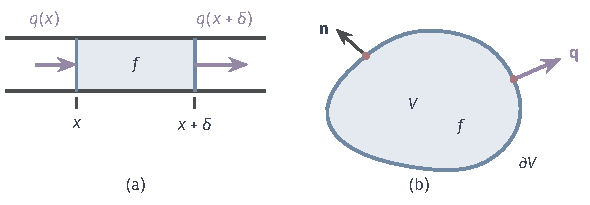
\includegraphics[width=100mm]{figures/06-differential-equations/02-partial-differential-equations/tikz/ellip-flux-balance/figure.pdf}
  \caption{热量收支平衡。(a)区间上的一小段：从左端流入$q(x)$，从右端流出$q(x+\delta)$，两者之差由段内的源项$f$补足。(b)多维区域中的控制体$V$：紫色箭头是热流$\bm{q}$，黑色箭头是边界的外法向$\bm{n}$，穿过$\partial V$的净流出量等于$V$内的总产热。}
  \label{fig:ellip-flux-balance}
\end{BookInlineFigure}

式~\eqref{eq:ellip-1d-equation}是二阶常微分方程，但它的提法与第~\ref{chap:ordinary-differential-equations}章的初值问题不同。初值问题在同一点给出$u$和$u'$，解可以从左向右递推。这里的两个条件分别放在区间的两端，右端的温度会影响左端，无法从一头推到另一头，必须把整段一起解出来。

取$a=1$、$f=1$，两端温度为零。方程$-u''=1$的解是
\begin{equation}
 u(x)=\frac{x(1-x)}{2},
 \label{eq:ellip-running-solution}
\end{equation}
它在中点取最大值$u(1/2)=1/8$。这个例子贯穿全章。后面每种方法算出的结果，都可以拿它来核对。

\paragraph{多维的散度型方程}
把收支平衡搬到区域$\Omega\subset\mathbb{R}^{d}$上。热流现在是向量场$\bm{q}(\bm{x})$，任取控制体$V\subset\Omega$，如图~\ref{fig:ellip-flux-balance}(b)，净流出量等于总产热：
\[
 \int_{\partial V}\bm{q}\cdot\bm{n}\,\mathrm{d}S=\int_Vf\,\mathrm{d}\bm{x} .
\]

由散度定理（可参考\BookChapterRef{chap:integral-theorems}{卷二第27章“积分定理”}），左端等于$\int_V\nabla\cdot\bm{q}\,\mathrm{d}\bm{x}$。这个等式对每个小控制体都成立，被积函数连续时可得$\nabla\cdot\bm{q}=f$。

导热率在不同方向上可能不同，例如木材顺纹与横纹导热差别很大，所以导热定律写成$\bm{q}=-\bm{A}(\bm{x})\nabla u$，其中$\bm{A}(\bm{x})$是$d\times d$的\term{扩散系数矩阵}（diffusion coefficient matrix）。于是得到散度型方程
\begin{equation}
 -\nabla\cdot\bigl(\bm{A}(\bm{x})\nabla u\bigr)=f\qquad\text{于}\ \Omega.
 \label{eq:ellip-divergence-form}
\end{equation}

取$\bm{A}=\bm{I}$，方程化为\term{Poisson方程}（Poisson equation）
\begin{equation}
 -\Delta u=f\qquad\text{于}\ \Omega,
 \label{eq:ellip-poisson}
\end{equation}
其中$\Delta u=\sum_{i=1}^d\partial_{i}^2u$是Laplace算子。$f=0$时称为Laplace方程，它的解称为\term{调和函数}（harmonic function）。方程前面的负号让$f>0$对应发热：$-\Delta u>0$表示$u$在该点附近比周围的平均值高，这正是热源处温度的样子。

第~\ref{chap:pde-problems}章按二阶项系数的符号结构区分方程类型：系数矩阵对称正定是椭圆型，还有一个时间方向上的一阶导数是抛物型，时间与空间的二阶导数异号是双曲型。式~\eqref{eq:ellip-divergence-form}没有时间，$\bm{A}$正定，就是椭圆型的典型代表。

\paragraph{三类边界条件}
方程只说明区域内部的收支，边界上发生什么要另外指定。设$\Omega$有界，$\bm{n}$是$\partial\Omega$上的外法向，$g$是边界上给定的函数。常用的条件有三类：

\begin{itemize}
 \item \term{Dirichlet边界条件}（Dirichlet boundary condition）$u=g$：边界温度由外界固定，如贴在恒温槽上。
 \item \term{Neumann边界条件}（Neumann boundary condition）$\bm{n}\cdot\bm{A}\nabla u=g$：规定穿过边界流入的热流。由$\bm{q}=-\bm{A}\nabla u$，$-\bm{q}\cdot\bm{n}$是单位面积上的流入量，$g=0$表示绝热。
 \item \term{Robin边界条件}（Robin boundary condition）$\bm{n}\cdot\bm{A}\nabla u+\beta u=g$，其中$\beta\geq0$：通过边界与环境换热，换热量正比于边界温度与环境温度之差，$g/\beta$相当于环境温度。
\end{itemize}

三者也可以分片出现在边界的不同部分。图~\ref{fig:ellip-boundary-types}固定源项$f=1$和左端$u(0)=0$，只改变右端的条件。绝热端把所有热量都存在棒内，温度最高；固定温度的右端可以直接散热，温度最低；Robin条件介于两者之间。

\begin{BookInlineFigure}
  \centering
  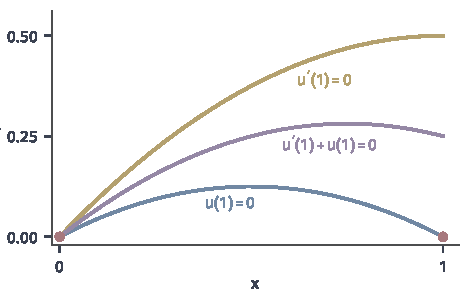
\includegraphics[width=80mm]{figures/06-differential-equations/02-partial-differential-equations/matplotlib/ellip-boundary-types/figure.pdf}
  \caption{同一方程$-u''=1$、同一左端条件$u(0)=0$，右端换三种条件。蓝线$u(1)=0$，解为$x(1-x)/2$；紫线$u'(1)+u(1)=0$，解为$3x/4-x^2/2$；黄线$u'(1)=0$，解为$x-x^2/2$。红点标出取定的边界值。}
  \label{fig:ellip-boundary-types}
\end{BookInlineFigure}

这三个解都可以手算验证。三者都有$-u''=1$和$u(0)=0$，因而都形如$u=Bx-x^2/2$，右端的条件只决定常数$B$：$u(1)=0$给出$B=1/2$，$u'(1)=0$给出$B=1$，$u'(1)+u(1)=0$即$(B-1)+(B-\tfrac12)=0$，给出$B=3/4$。

\paragraph{一致椭圆系数}
后面所有定理都要用到$\bm{A}$的一条性质。在式~\eqref{eq:ellip-divergence-form}两边乘以$u$并积分，会出现二次量$\int\nabla u^\top\bm{A}\nabla u$，它衡量的是梯度带来的能量。我们要求这个量能够控制梯度本身的大小，并且系数不能大到无界。

\begin{definition}[一致椭圆]
\label{def:ellip-uniform}
设$\bm{A}:\Omega\to\mathbb{R}^{d\times d}$可测。若存在常数$0<\kappa_{\min}\leq\kappa_{\max}<\infty$，使几乎所有$\bm{x}\in\Omega$和所有$\bm{\xi}\in\mathbb{R}^{d}$满足
\begin{equation}
 \bm{\xi}^\top\bm{A}(\bm{x})\bm{\xi}\geq\kappa_{\min}\lVert\bm{\xi}\rVert_2^2,\qquad
 \lVert\bm{A}(\bm{x})\bm{\xi}\rVert_2\leq\kappa_{\max}\lVert\bm{\xi}\rVert_2,
 \label{eq:ellip-uniform}
\end{equation}
就称$\bm{A}$在$\Omega$上\term{一致椭圆}（uniformly elliptic）。
\end{definition}

定义不要求$\bm{A}$连续，也不要求对称。系数可以在两种材料的交界处跳变，这在应用中很常见。若$\bm{A}$对称，第一个条件说$\bm{A}(\bm{x})$的最小特征值不小于$\kappa_{\min}$，第二个条件说最大特征值不超过$\kappa_{\max}$。

对任意足够光滑的$u$，取$\bm{\xi}=\nabla u(\bm{x})$，再对$\bm{x}$积分，得到
\begin{equation}
 \int_\Omega\nabla u^\top\bm{A}\nabla u\,\mathrm{d}\bm{x}\geq\kappa_{\min}\int_\Omega\lVert\nabla u\rVert_2^2\,\mathrm{d}\bm{x}.
 \label{eq:ellip-gradient-control}
\end{equation}
这就是一致椭圆的用途：无论梯度指向哪个方向，都有不低于$\kappa_{\min}$的“导热能力”把它计入能量。

图~\ref{fig:ellip-ellipticity}用集合$\{\bm{\xi}:\bm{\xi}^\top\bm{A}\bm{\xi}=1\}$的形状区分三种情况。(a)中$\bm{A}$的元素是$2,0.6,0.6,1$，特征值约为$2.28$和$0.72$，水平集是夹在两个圆之间的椭圆，这是椭圆一词的来历。

(b)中$\bm{A}=\operatorname{diag}(1,0)$，$\xi_2$方向的梯度完全不被计入，能量控制不住这个方向，方程在$x_2$方向没有扩散，这是退化情形。(c)中$\bm{A}=\operatorname{diag}(1,-1)$不定，水平集是双曲线，二次量可以取负，这是波动方程的结构，第~\ref{chap:wave-equations}章要用完全不同的方法处理。

\begin{BookInlineFigure}
  \centering
  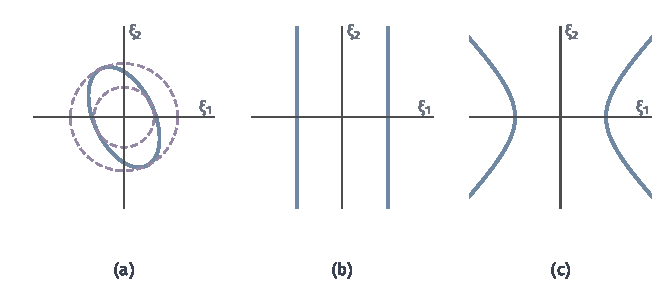
\includegraphics[width=112mm]{figures/06-differential-equations/02-partial-differential-equations/matplotlib/ellip-ellipticity/figure.pdf}
  \caption{水平集$\bm{\xi}^\top\bm{A}\bm{\xi}=1$（蓝线）的三种形状。(a)一致椭圆：椭圆被夹在半径$\kappa_{\max}^{-1/2}$与$\kappa_{\min}^{-1/2}$的两个圆（紫色虚线）之间。(b)退化：$\bm{A}=\operatorname{diag}(1,0)$，水平集是两条平行线，$\xi_2$方向无界。(c)不定：$\bm{A}=\operatorname{diag}(1,-1)$，水平集是双曲线。}
  \label{fig:ellip-ellipticity}
\end{BookInlineFigure}

要注意，主部一致椭圆只说明最高阶项的结构。方程$-\Delta u-k^2u=f$的二阶项与Poisson方程相同，零阶项的符号却相反，它在某些$k$上会失去唯一性，后面的结论不能照搬。本章的主线是式~\eqref{eq:ellip-divergence-form}，低阶项在用到时单独说明条件。


\section{解的表示}
\label{sec:ellip-representation}

能把解写成公式的情形不多，但它们最能说明解由什么决定。下面三种表示各借助一种结构：区间上可以直接积分，线性性允许把点源的响应叠加起来，自伴性允许沿特征函数分解。每个公式都有成立的前提，这些前提与公式一起说明。

\subsection{区间上的求解}
\label{sec:ellip-interval}

先看最简单的两点边值问题。给定$f\in C[0,1]$与边界值$g_0,g_1$，求$u\in C^2[0,1]$满足
\begin{equation}
 -u''=f\quad\text{于}\ (0,1),\qquad u(0)=g_0,\quad u(1)=g_1.
 \label{eq:ellip-interval-dirichlet}
\end{equation}

积分一次，$u'(0)$是一个待定常数，记为$C_1$：
\[
 u'(x)=C_1-\int_0^xf(s)\,\mathrm{d}s .
\]
再积分一次，把二重积分交换次序化成单重积分，$u(0)$是第二个常数：
\[
 u(x)=u(0)+C_1x-\int_0^x(x-s)f(s)\,\mathrm{d}s .
\]

代入左端条件，得到$u(0)=g_0$。代入右端条件，解出$C_1$：
\[
 C_1=g_1-g_0+\int_0^1(1-s)f(s)\,\mathrm{d}s .
\]

两个积分常数恰好被两个边界条件确定。代回去整理，解分成两部分：
\begin{equation}
 u(x)=\underbrace{g_0(1-x)+g_1x}_{\text{边界贡献}}
 +\underbrace{x\int_0^1(1-s)f(s)\,\mathrm{d}s-\int_0^x(x-s)f(s)\,\mathrm{d}s}_{\text{源项贡献}} .
 \label{eq:ellip-interval-solution}
\end{equation}

边界贡献是连接两个边界值的直线，满足$u''=0$。源项贡献在两端为零。这一分解来自线性：边界数据和源项可以分别处理，再把结果相加。

取$f=1$、$g_0=1$、$g_1=3$做一次手算。式~\eqref{eq:ellip-interval-solution}中的积分是
\[
 \int_0^1(1-s)\,\mathrm{d}s=\frac12,\qquad \int_0^x(x-s)\,\mathrm{d}s=\frac{x^2}2 .
\]
于是
\[
 u(x)=(1+2x)+\frac{x}{2}-\frac{x^2}{2}=1+2x+\frac{x(1-x)}{2},
\]
边界贡献是$1+2x$，源项贡献正是式~\eqref{eq:ellip-running-solution}。

唯一性也可以直接读出。若$u_1,u_2$都是解，差$w=u_1-u_2$满足$w''=0$和$w(0)=w(1)=0$。$w''=0$说明$w$是一次函数，两端为零的一次函数只能恒为零。

\paragraph{Neumann条件：相容性与不唯一}
把两端的条件都换成通量。按上一节的约定，外法向在$x=0$处指向左，在$x=1$处指向右，所以问题是
\begin{equation}
 -u''=f\quad\text{于}\ (0,1),\qquad -u'(0)=g_0,\quad u'(1)=g_1.
 \label{eq:ellip-interval-neumann}
\end{equation}
仍然积分一次，这次两端的条件都落在$u'$上，$u$本身一次也没有被约束。

对方程在$[0,1]$上积分，由牛顿--莱布尼茨公式，
\[
 \int_0^1f\,\mathrm{d}x=-u'(1)+u'(0)=-g_1-g_0 .
\]
也就是说，解若存在，数据必须满足
\begin{equation}
 \int_0^1f\,\mathrm{d}x+g_0+g_1=0.
 \label{eq:ellip-interval-compat}
\end{equation}

物理上这是总热量的收支：棒内总产热加上从两端流入的热量必须为零，否则温度不可能稳定。这样的条件称为\term{相容条件}（compatibility condition）。反过来，式~\eqref{eq:ellip-interval-compat}成立时，由$u'(x)=-g_0-\int_0^xf$定义的函数在$x=1$处恰好满足第二个条件，再积分一次就得到解，积分常数$c$可以任取。

取$f(x)=1-2x$，$g_0=g_1=0$。此时$\int_0^1f=0$，相容条件成立。积分得到
\[
 u'(x)=x^2-x,\qquad u(x)=\frac{x^3}{3}-\frac{x^2}{2}+c .
\]
图~\ref{fig:ellip-neumann-compat}(a)是不同$c$对应的解。整条曲线可以上下平移，因为方程和边界条件都只看导数。若要挑出一个代表，可以要求$\int_0^1u=0$，由$\int_0^1(x^3/3-x^2/2)\,\mathrm{d}x=-1/12$得到$c=1/12$。

\begin{BookInlineFigure}
  \centering
  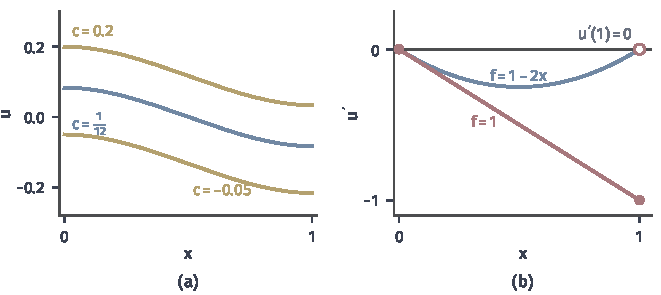
\includegraphics[width=112mm]{figures/06-differential-equations/02-partial-differential-equations/matplotlib/ellip-neumann-compat/figure.pdf}
  \caption{区间上的Neumann问题，$g_0=g_1=0$。(a)$f=1-2x$满足相容条件，解$x^3/3-x^2/2+c$可以任意平移；蓝线是零均值的代表，黄线是另外两个常数。(b)$u'$从$u'(0)=0$（红点）出发：$f=1-2x$时蓝线回到$u'(1)=0$（空心点）；$f=1$时红线走到$-1$，右端条件无法满足。}
  \label{fig:ellip-neumann-compat}
\end{BookInlineFigure}

若取$f=1$，图~\ref{fig:ellip-neumann-compat}(b)显示了失败的方式。从$u'(0)=0$出发，$u'(x)=-x$到右端变成$-1$，而边界要求$0$。两端绝热，棒内持续发热，温度只会不断上升，稳态根本不存在。

对比两种边界条件：Dirichlet问题对任何$f$都唯一可解，Neumann问题只在数据满足一个线性约束时可解，可解时解有一维的自由度。这与线性方程组$\bm{K}\bm{c}=\bm{b}$在$\bm{K}$奇异时的情形相同，后面会把这个对应写清楚。

\subsection{Green函数}
\label{sec:ellip-green}

式~\eqref{eq:ellip-interval-solution}中源项的贡献是对$f$的积分，说明解线性地依赖于$f$。线性依赖应该能写成“每一处的源乘以一个响应，再叠加”。这个响应是什么？

\paragraph{矩阵的逆给出点源响应}
把函数看成长向量，问题就变成矩阵方程。将$[0,1]$等分为$n+1$段，步长$h=1/(n+1)$，内部格点$x_i=ih$。用二阶差商近似$-u''$，边界值为零，得到$\bm{K}\bm{u}=\bm{f}$，其中
\begin{equation}
 \bm{K}=\frac1{h^2}\begin{pmatrix}2&-1&&\\-1&2&\ddots&\\&\ddots&\ddots&-1\\&&-1&2\end{pmatrix}.
 \label{eq:ellip-discrete-laplacian}
\end{equation}

解是$\bm{u}=\bm{K}^{-1}\bm{f}$，写成分量为$u_i=\sum_j(\bm{K}^{-1})_{i,j}f_j$。$\bm{K}^{-1}$的第$j$列，就是只在第$j$个格点放单位源时的整个解。求逆等于把每个格点上的点源响应都算好。

取$n=3$，$h=1/4$，可以手算：
\[
 \bm{K}=16\begin{pmatrix}2&-1&0\\-1&2&-1\\0&-1&2\end{pmatrix},\qquad
 \bm{K}^{-1}=\frac1{64}\begin{pmatrix}3&2&1\\2&4&2\\1&2&3\end{pmatrix}.
\]
每一列先升后降，顶点在对角元处，折线形如帐篷。矩阵对称，说明$y$处放源在$x$处的响应，等于$x$处放源在$y$处的响应。

\paragraph{区间上的点源}
让格点加密，这些帐篷收敛到什么？连续地提问：在$y\in(0,1)$处放一个单位点源，解$G(\cdot,y)$应当满足什么？点源之外没有源，所以$G(\cdot,y)$在$(0,y)$和$(y,1)$上都满足$u''=0$，都是一次函数。加上两端为零，可设
\[
 G(x,y)=\begin{cases}\alpha x,&0\leq x\leq y,\\ \gamma(1-x),&y\leq x\leq1 .\end{cases}
\]

在$y$处需要两个条件。第一，温度连续，否则温度有跳变，热流无穷大，这就是$\alpha y=\gamma(1-y)$。第二，把$-u''=f$在包含$y$的小区间上积分，右端是单位源的总量$1$，左端是$u'$在左右两侧之差的相反数，所以$u'$在$y$处向下跳$1$，这就是$\alpha+\gamma=1$。

两个方程解出$\alpha=1-y$，$\gamma=y$。于是
\begin{equation}
 G(x,y)=\begin{cases}x(1-y),&0\leq x\leq y,\\ y(1-x),&y\leq x\leq1 .\end{cases}
 \label{eq:ellip-green-1d}
\end{equation}
它称为这个边值问题的\term{Green函数}（Green's function）。第~\ref{chap:linear-differential-systems}章也有一个积分核，把脉冲输入变成后续响应，它在脉冲发生之前为零，体现因果。这里的$G$在点源两侧都不为零，因为边界条件把信息从两个方向都传了过来。

有了点源响应，一般的源就是点源的叠加：
\begin{equation}
 u(x)=\int_0^1G(x,y)f(y)\,\mathrm{d}y .
 \label{eq:ellip-green-1d-rep}
\end{equation}
图~\ref{fig:ellip-inverse-tent}验证了矩阵与函数的对应，$\bm{K}^{-1}$除以$h$后，每列的元素恰好落在$G$上。图~\ref{fig:ellip-tents-superposition}展示叠加：几个点源的帐篷相加，点源越多越接近真解。

\begin{BookInlineFigure}
  \centering
  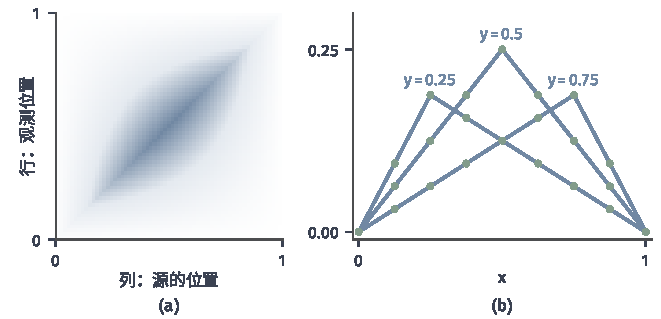
\includegraphics[width=112mm]{figures/06-differential-equations/02-partial-differential-equations/matplotlib/ellip-inverse-tent/figure.pdf}
  \caption{差分矩阵的逆是离散的Green函数。(a)$n=63$时$\bm{K}^{-1}/h$的取值，颜色越深值越大，沿对角线形成山脊。(b)$n=7$时第$2,4,6$列的元素（绿点）与式~\eqref{eq:ellip-green-1d}的$G(\cdot,y)$（蓝线），在格点上数值完全相同。}
  \label{fig:ellip-inverse-tent}
\end{BookInlineFigure}

现在验证式~\eqref{eq:ellip-green-1d-rep}。把积分在$y=x$处拆开，代入式~\eqref{eq:ellip-green-1d}：
\[
 u(x)=(1-x)\int_0^xyf(y)\,\mathrm{d}y+x\int_x^1(1-y)f(y)\,\mathrm{d}y .
\]

对$x$求导，积分限上出现的两项是$(1-x)xf(x)$和$-x(1-x)f(x)$，互相抵消，只剩
\[
 u'(x)=-\int_0^xyf(y)\,\mathrm{d}y+\int_x^1(1-y)f(y)\,\mathrm{d}y .
\]

再求导，得到
\[
 u''(x)=-xf(x)-(1-x)f(x)=-f(x).
\]
又由公式直接读出$u(0)=u(1)=0$。取$f=1$，
\[
 u(x)=(1-x)\frac{x^2}{2}+x\frac{(1-x)^2}{2}=\frac{x(1-x)}{2},
\]
这正是式~\eqref{eq:ellip-running-solution}。

\begin{BookInlineFigure}
  \centering
  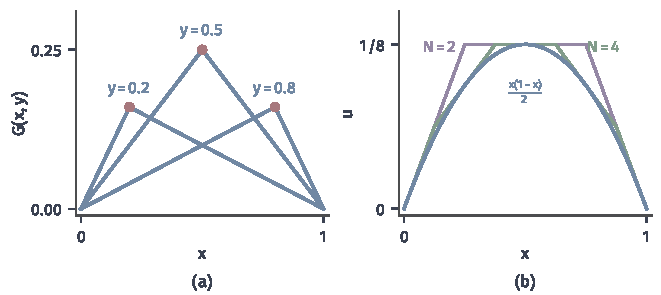
\includegraphics[width=112mm]{figures/06-differential-equations/02-partial-differential-equations/matplotlib/ellip-tents-superposition/figure.pdf}
  \caption{点源响应的叠加。(a)三个位置$y$处的单位点源产生的帐篷$G(\cdot,y)$，红点是顶点$(y,y(1-y))$。(b)均匀源$f=1$的离散近似：在$N$个等分小段的中点放权重$1/N$的点源，紫线$N=2$，绿线$N=4$，$N$增大时趋于蓝线$x(1-x)/2$。}
  \label{fig:ellip-tents-superposition}
\end{BookInlineFigure}

\paragraph{全空间的基本解}
多维情形不能分段积分，但点源响应的想法仍然有效。先在没有边界的全空间里问：单位点源在原点产生的平衡温度是什么？

对称性告诉我们解只依赖于到原点的距离$r=\lVert\bm{x}\rVert_2$，记为$\varphi(r)$。把所有热量想成从原点向外流：稳态下，单位热源产生的热量必须全部穿过每一个以原点为心的球面。半径$r$的球面面积是$d\omega_dr^{d-1}$，其中$\omega_d$是单位球的体积。所以径向热流密度为
\[
 -\varphi'(r)=\frac1{d\omega_dr^{d-1}} .
\]

积分一次，常数取最简单的值，就得到\termalias{基本解-偏微分方程}{基本解}（fundamental solution）
\begin{equation}
 \Phi(\bm{x})=\begin{cases}
 -\dfrac{\lVert\bm{x}\rVert_2}{2},&d=1,\\
 -\dfrac1{2\pi}\log\lVert\bm{x}\rVert_2,&d=2,\\
 \dfrac1{d(d-2)\omega_d}\,\lVert\bm{x}\rVert_2^{2-d},&d\geq3 .
 \end{cases}
 \label{eq:ellip-fundamental}
\end{equation}
$d=3$时$\omega_3=4\pi/3$，$\Phi=1/(4\pi\lVert\bm{x}\rVert_2)$。直接计算可知$\Delta\Phi=0$在原点之外成立：径向函数的Laplace是$r^{1-d}(r^{d-1}\varphi')'$，而$r^{d-1}\varphi'$是常数。

图~\ref{fig:ellip-fundamental-radial}比较了三个维数。维数越高，球面面积随半径增长越快，同样的热量摊得越薄，所以(b)中的流密度衰减得越快。$d=1$时热流不衰减，$\Phi$一直线性下降；$d\geq3$时$\Phi$在无穷远趋于零；$d=2$介于两者之间，$\Phi$对数发散。

\begin{BookInlineFigure}
  \centering
  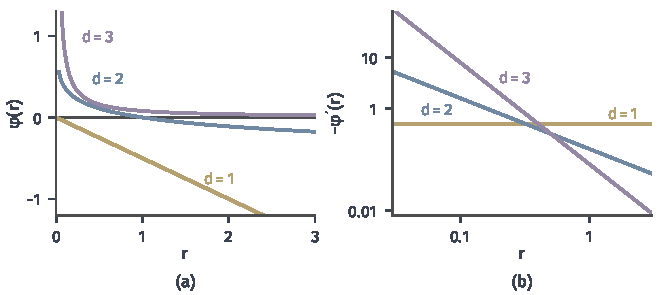
\includegraphics[width=112mm]{figures/06-differential-equations/02-partial-differential-equations/matplotlib/ellip-fundamental-radial/figure.pdf}
  \caption{基本解的径向形状。(a)$\varphi(r)$：$d=1$（黄）是直线，$d=2$（蓝）是对数，$d=3$（紫）是$1/(4\pi r)$，$d\geq2$时在原点发散。(b)流密度$-\varphi'(r)$的双对数图，斜率分别为$0,-1,-2$，体现单位热量摊在面积$d\omega_dr^{d-1}$上。}
  \label{fig:ellip-fundamental-radial}
\end{BookInlineFigure}

基本解只回答了全空间的问题。对紧支撑的$C^2$函数$f$，卷积
\[
 v(\bm{x})=\int_{\mathbb{R}^{d}}\Phi(\bm{x}-\bm{y})f(\bm{y})\,\mathrm{d}\bm{y}
\]
满足$-\Delta v=f$，这在下面的表示定理之后就能验证。但$v$不满足任何给定的边界条件。在$(0,1)$上取$f=1$，
\[
 v(x)=-\int_0^1\frac{\lvert x-y\rvert}{2}\,\mathrm{d}y=-\frac{x^2+(1-x)^2}{4},
\]
边界值$v(0)=v(1)=-1/4$不是$0$。它比真解$x(1-x)/2$处处低$1/4$，必须修正。

\paragraph{表示公式}
要知道边界怎样影响解，用Green第二恒等式。设$V$是有界区域，$\partial V$足够光滑，$u,w\in C^2(\overline V)$。向量场$u\nabla w-w\nabla u$的散度是
\[
 \nabla\cdot(u\nabla w-w\nabla u)=u\Delta w-w\Delta u .
\]
对它用散度定理，得到
\begin{equation}
 \int_V(u\Delta w-w\Delta u)\,\mathrm{d}\bm{x}=\int_{\partial V}(u\,\partial_{\bm{n}}w-w\,\partial_{\bm{n}}u)\,\mathrm{d}S,
 \label{eq:ellip-green-second}
\end{equation}
其中$\partial_{\bm{n}}w=\bm{n}\cdot\nabla w$是外法向导数。

我们想取$w=\Phi(\bm{x}-\cdot)$，但它在$\bm{x}$处奇异。办法是挖掉以$\bm{x}$为中心的小球，见图~\ref{fig:ellip-excised-ball}，在剩下的区域用恒等式，再让球缩小。

\begin{BookInlineFigure}
  \centering
  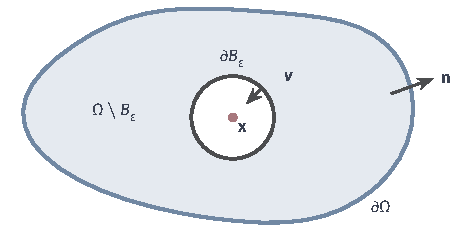
\includegraphics[width=78mm]{figures/06-differential-equations/02-partial-differential-equations/tikz/ellip-excised-ball/figure.pdf}
  \caption{挖去小球后的区域$\Omega\setminus B_\varepsilon$。外边界上的法向$\bm{n}$指向区域外，小球面上区域的外法向$\bm{\nu}$指向球心$\bm{x}$。}
  \label{fig:ellip-excised-ball}
\end{BookInlineFigure}

\begin{theorem}[Green表示公式]
\label{thm:ellip-representation}
设$d\geq2$，$\Omega\subset\mathbb{R}^{d}$是边界光滑的有界区域，$u\in C^2(\overline\Omega)$。则对每个$\bm{x}\in\Omega$，
\begin{equation}
 \begin{aligned}
 u(\bm{x})={}&\int_\Omega\Phi(\bm{x}-\bm{y})\bigl(-\Delta u(\bm{y})\bigr)\,\mathrm{d}\bm{y}\\
 &+\int_{\partial\Omega}\Bigl(\Phi(\bm{x}-\bm{y})\,\partial_{\bm{n}}u(\bm{y})-u(\bm{y})\,\partial_{\bm{n}}\Phi(\bm{x}-\bm{y})\Bigr)\,\mathrm{d}S(\bm{y}),
 \end{aligned}
 \label{eq:ellip-representation}
\end{equation}
其中法向导数对变量$\bm{y}$求。
\end{theorem}

\begin{proof}
固定$\bm{x}$，记$w(\bm{y})=\Phi(\bm{x}-\bm{y})$，取$\varepsilon$足够小使$\overline{B_\varepsilon(\bm{x})}\subset\Omega$，令$V=\Omega\setminus\overline{B_\varepsilon(\bm{x})}$。在$V$上$\Delta w=0$，式~\eqref{eq:ellip-green-second}化为
\[
 -\int_Vw\Delta u\,\mathrm{d}\bm{y}=\int_{\partial\Omega}(u\,\partial_{\bm{n}}w-w\,\partial_{\bm{n}}u)\,\mathrm{d}S+\int_{\partial B_\varepsilon}(u\,\partial_{\bm{\nu}}w-w\,\partial_{\bm{\nu}}u)\,\mathrm{d}S .
\]

在小球面上，$\bm{\nu}$指向球心，$w$的值是$\varphi(\varepsilon)$，方向导数是
\[
 \partial_{\bm{\nu}}w=-\varphi'(\varepsilon)=\frac1{d\omega_d\varepsilon^{d-1}},
\]
它正好是球面面积的倒数。于是第一项是$u$在球面上的平均值：
\[
 \int_{\partial B_\varepsilon}u\,\partial_{\bm{\nu}}w\,\mathrm{d}S=\frac1{\lvert\partial B_\varepsilon\rvert}\int_{\partial B_\varepsilon}u\,\mathrm{d}S\ \longrightarrow\ u(\bm{x}),\qquad\varepsilon\to0,
\]
极限成立是因为$u$连续。

第二项的绝对值不超过$\lvert\varphi(\varepsilon)\rvert\cdot d\omega_d\varepsilon^{d-1}\cdot\max\lVert\nabla u\rVert_2$。$d=2$时这是$\varepsilon\lvert\log\varepsilon\rvert$的倍数，$d\geq3$时是$\varepsilon$的倍数，都趋于零。

最后，$\Phi(\bm{x}-\cdot)$在$\bm{x}$附近可积，$\Delta u$有界，左端的积分当$\varepsilon\to0$时收敛到$\int_\Omega w\Delta u$的相反数。三个极限合起来，移项即得式~\eqref{eq:ellip-representation}。
\end{proof}

现在可以补上卷积的验证。设$f\in C_c^2(\mathbb{R}^{d})$，把导数放到$f$上，有$\Delta v=\Phi*\Delta f$。把定理用于$u=f$、足够大的球$\Omega$，边界项为零，给出$f=\Phi*(-\Delta f)$，所以$-\Delta v=f$。

式~\eqref{eq:ellip-representation}还不能算是解的公式，因为右端同时用到了边界上的$u$和$\partial_{\bm{n}}u$。对Dirichlet问题，$\partial_{\bm{n}}u$恰恰是未知的。要把它消掉。

\paragraph{区域的Green函数}
办法是给基本解加一个调和的修正，使修正后的函数在边界上为零，这样含$\partial_{\bm{n}}u$的项就消失了。

\begin{definition}[区域的Green函数]
\label{def:ellip-green-domain}
设$\Omega$是有界区域。若对每个$\bm{x}\in\Omega$，存在$h^{\bm{x}}\in C^2(\overline\Omega)$满足$\Delta h^{\bm{x}}=0$，且在$\partial\Omega$上$h^{\bm{x}}(\bm{y})=\Phi(\bm{x}-\bm{y})$，则称
\begin{equation}
 G(\bm{x},\bm{y})=\Phi(\bm{x}-\bm{y})-h^{\bm{x}}(\bm{y})
 \label{eq:ellip-green-domain}
\end{equation}
为$\Omega$上Dirichlet问题的Green函数。
\end{definition}

$\Phi$负责在点源处产生正确的奇性，$h^{\bm{x}}$负责抵消边界值。图~\ref{fig:ellip-green-corrector}在一维展示了这个构造：黄色的基本解在两端不为零，紫色的修正是过这两个端点值的直线，两者相减就是蓝色的帐篷。$\Phi$在全空间只有一个，而$G$随着区域变化，换一个区域就要重新解一次修正问题。

\begin{BookInlineFigure}
  \centering
  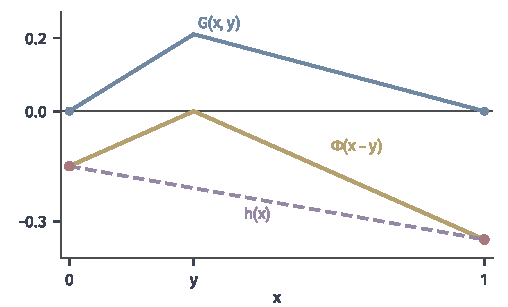
\includegraphics[width=86mm]{figures/06-differential-equations/02-partial-differential-equations/matplotlib/ellip-green-corrector/figure.pdf}
  \caption{一维Green函数的构造，$y=0.3$。黄线是基本解$\Phi(x-y)=-\lvert x-y\rvert/2$，红点是它的两个端点值。紫色虚线$h$是以这两个值为端点的直线，$h''=0$。蓝线$G=\Phi-h$在两端为零，就是式~\eqref{eq:ellip-green-1d}。}
  \label{fig:ellip-green-corrector}
\end{BookInlineFigure}

用$u$和$h^{\bm{x}}$再做一次式~\eqref{eq:ellip-green-second}，由$\Delta h^{\bm{x}}=0$得到
\[
 \int_\Omega h^{\bm{x}}\bigl(-\Delta u\bigr)\,\mathrm{d}\bm{y}=\int_{\partial\Omega}\bigl(u\,\partial_{\bm{n}}h^{\bm{x}}-h^{\bm{x}}\,\partial_{\bm{n}}u\bigr)\,\mathrm{d}S .
\]

用式~\eqref{eq:ellip-representation}减去这个等式。在边界上$\Phi=h^{\bm{x}}$，含$\partial_{\bm{n}}u$的两项抵消，得到
\begin{equation}
 u(\bm{x})=\int_\Omega G(\bm{x},\bm{y})\bigl(-\Delta u(\bm{y})\bigr)\,\mathrm{d}\bm{y}-\int_{\partial\Omega}u(\bm{y})\,\partial_{\bm{n}}G(\bm{x},\bm{y})\,\mathrm{d}S(\bm{y}) .
 \label{eq:ellip-green-rep}
\end{equation}

这个公式把解分成两份，第一份由源项产生，第二份由边界值产生。边界贡献不能省略，否则非零边值的信息就丢了。一维的验证很直接：端点$y=0$的外法向指向左，$\partial_{\bm{n}}G=-\partial_yG(x,0)=-(1-x)$，边界项给出$g_0(1-x)$；同样$y=1$处给出$g_1x$。两项合起来就是式~\eqref{eq:ellip-interval-solution}中的那条直线。

要小心公式的逻辑方向。式~\eqref{eq:ellip-green-rep}是说：\emph{如果}$C^2(\overline\Omega)$的解存在，\emph{并且}Green函数存在且足够光滑，解就必须是这个样子。它推出了唯一性，但没有证明存在性。

\paragraph{像源法}
几何特别简单时，修正项可以直接猜出来。考虑上半平面$\{x_2>0\}$，点源在$\bm{y}=(y_1,y_2)$。在边界另一侧的镜像点$\bm{y}^{*}=(y_1,-y_2)$放一个负的点源，由对称性，边界$x_2=0$上每一点到$\bm{y}$与到$\bm{y}^{*}$的距离相等，两个势在边界上抵消。这种做法称为\term{像源法}（method of images），二维的Green函数是
\begin{equation}
 G(\bm{x},\bm{y})=-\frac1{2\pi}\bigl(\log\lVert\bm{x}-\bm{y}\rVert_2-\log\lVert\bm{x}-\bm{y}^{*}\rVert_2\bigr).
 \label{eq:ellip-green-half-plane}
\end{equation}

半平面的外法向是$-\bm{e}_2$，把$-\partial_{\bm{n}}G=\partial_{y_2}G$在$y_2=0$处算出来：
\[
 P(\bm{x},y_1)=\frac{x_2}{\pi\bigl((x_1-y_1)^2+x_2^2\bigr)} .
\]
边界数据$g$产生的解是
\[
 u(\bm{x})=\int_{\mathbb{R}}P(\bm{x},y_1)\,g(y_1)\,\mathrm{d}y_1 ,
\]
$P$称为半平面的\term{Poisson核}（Poisson kernel）。半平面无界，这个公式对有界连续的$g$给出有界调和函数，要证明解确实取到边界值，需要对$P$的集中性质单独做极限估计，这里不细述。

图~\ref{fig:ellip-image-method}(b)说明Poisson核是一个加权平均：离边界越近，权重越集中在最近的边界点附近。这与解的边值恰好是$g$相吻合。离边界越远，权重摊得越开，解越光滑。

\begin{BookInlineFigure}
  \centering
  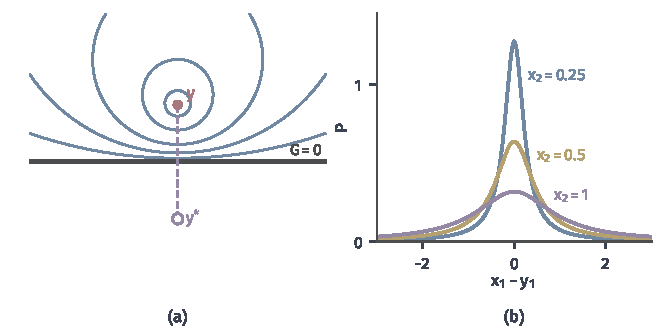
\includegraphics[width=112mm]{figures/06-differential-equations/02-partial-differential-equations/matplotlib/ellip-image-method/figure.pdf}
  \caption{上半平面的Green函数。(a)红点$\bm{y}=(0,1)$是点源，紫色空心点$\bm{y}^{*}=(0,-1)$是虚设的负像源，蓝线是$G$的等值线，粗线是边界，边界上$G=0$。(b)Poisson核$P$随$x_1-y_1$的变化，$x_2$越小峰越尖；每条曲线下的面积都是$1$。}
  \label{fig:ellip-image-method}
\end{BookInlineFigure}

\subsection{谱展开}
\label{sec:ellip-spectral}

Green函数把解写成“一处一处”的叠加。另一种思路是“一个模式一个模式”地叠加：找一组基，使微分算子在这组基下成为对角的，求解就成了逐个系数的除法。这正是对称矩阵的做法。

\paragraph{从矩阵的对角化到函数}
若$\bm{K}$对称正定，$\bm{K}=\bm{Q}\bm{\Lambda}\bm{Q}^\top$，那么$\bm{K}\bm{u}=\bm{f}$的解是把$\bm{f}$在特征向量上分解，每个分量除以对应的特征值，再合成。连续的对应物是
\begin{equation}
 -\Delta e_k=\lambda_ke_k\quad\text{于}\ \Omega,\qquad e_k=0\quad\text{于}\ \partial\Omega .
 \label{eq:ellip-eigenproblem}
\end{equation}

在区间$(0,1)$上，满足这个问题的函数和特征值是
\[
 e_k(x)=\sqrt2\sin(k\pi x),\qquad\lambda_k=k^2\pi^2,\qquad k\geq1 .
\]
这组函数是$L^2(0,1)$的标准正交基，它与Fourier级数的完备性同源，可参考\BookChapterRef{chap:fourier-transform}{卷四第14章“Fourier变换”}。把$f$与$u$按这组基展开，系数记为$f_k=\langle f,e_k\rangle$，$u_k=\langle u,e_k\rangle$。

用$e_k$乘方程$-u''=f$并积分，分部积分两次。$u$和$e_k$在端点都为零，边界项消失，得到
\[
 f_k=\int_0^1(-u'')e_k\,\mathrm{d}x=\int_0^1u(-e_k'')\,\mathrm{d}x=\lambda_ku_k .
\]
于是
\begin{equation}
 u=\sum_{k\geq1}\frac{f_k}{\lambda_k}\,e_k .
 \label{eq:ellip-spectral-solution}
\end{equation}

这个过程用到了边界条件的自伴结构：分部积分时$u$和$e_k$的边界项同时消失，$-\mathrm{d}^2/\mathrm{d}x^2$才能从$u$移到$e_k$上。对一般的有界区域，这样一组基是否存在，要等弱解理论建立之后才能回答。

\paragraph{一个完整的计算}
继续用$f=1$。系数是
\[
 f_k=\sqrt2\int_0^1\sin(k\pi x)\,\mathrm{d}x=\frac{\sqrt2\,(1-(-1)^k)}{k\pi} .
\]
偶数$k$的系数为零，奇数$k$的系数为$2\sqrt2/(k\pi)$。代入式~\eqref{eq:ellip-spectral-solution}，
\[
 u(x)=\sum_{k\ \text{奇}}\frac{4}{k^3\pi^3}\sin(k\pi x).
\]

在中点$x=1/2$处算几项部分和。$\sin(k\pi/2)$对$k=1,3,5$依次是$1,-1,1$，于是
\[
 \frac4{\pi^3}\approx0.12901,\qquad
 \frac4{\pi^3}\Bigl(1-\frac1{27}\Bigr)\approx0.12423,\qquad
 \frac4{\pi^3}\Bigl(1-\frac1{27}+\frac1{125}\Bigr)\approx0.12526 ,
\]
正在收敛到式~\eqref{eq:ellip-running-solution}给出的$1/8=0.125$。

图~\ref{fig:ellip-modes-coeffs}对比了$f$与$u$的系数。$f_k$按$1/k$衰减，所以部分和在间断处有明显的振荡，这是$f$在端点从$1$跳到边界值$0$的结果。$u_k=f_k/\lambda_k$按$1/k^3$衰减，只取第一项就已经和真解很接近。

除以$\lambda_k$压低高频，这就是椭圆问题的光滑作用。解比数据多出两阶导数的正则性，这在系数上表现为多出$k^{-2}$的衰减。

\begin{BookInlineFigure}
  \centering
  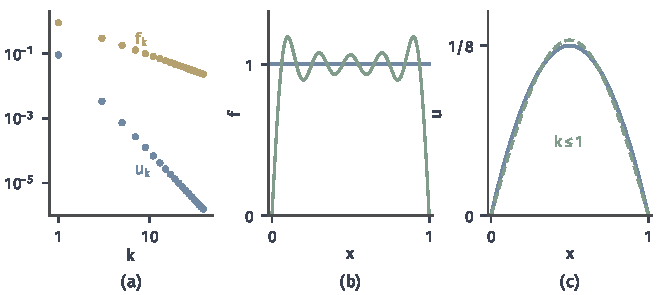
\includegraphics[width=112mm]{figures/06-differential-equations/02-partial-differential-equations/matplotlib/ellip-modes-coeffs/figure.pdf}
  \caption{$f=1$的正弦展开。(a)奇数$k$上$f_k$（黄）与$u_k=f_k/\lambda_k$（蓝）的双对数图，衰减率分别是$k^{-1}$与$k^{-3}$。(b)$f$的$k\leq9$部分和（绿）在$f$的目标值（蓝）附近振荡。(c)$u$的第一项（绿色虚线）已贴近真解（蓝）。}
  \label{fig:ellip-modes-coeffs}
\end{BookInlineFigure}

$f\in L^2(0,1)$时，式~\eqref{eq:ellip-spectral-solution}在$L^2$意义下收敛，它的导数级数也在$L^2$中收敛，这由下面两个有限的和保证：
\[
 \sum_k\frac{f_k^2}{\lambda_k^2}\leq\frac1{\lambda_1^2}\sum_kf_k^2<\infty,\qquad
 \sum_k\lambda_ku_k^2=\sum_k\frac{f_k^2}{\lambda_k}<\infty .
\]
逐点收敛和逐项求二阶导需要$f$有更多的光滑性，不能仅凭$f\in L^2$断言。

把$u_k=f_k/\lambda_k$的定义代回，再交换求和与积分，还能读出Green函数的谱表示：
\begin{equation}
 G(x,y)=\sum_{k\geq1}\frac{e_k(x)\,e_k(y)}{\lambda_k},
 \label{eq:ellip-green-spectral}
\end{equation}
这是矩阵等式$\bm{K}^{-1}=\sum_k\bm{q}_k\bm{q}_k^\top/\lambda_k$的函数版本。两种表示说的是同一个算子，一个按位置分解，一个按频率分解。

\paragraph{矩形区域}
积分区域是矩形时，变量分离给出二维的特征函数。在单位正方形上，
\[
 e_{m,n}(x_1,x_2)=2\sin(m\pi x_1)\sin(n\pi x_2),\qquad \lambda_{m,n}=\pi^2(m^2+n^2).
\]

若$f$恰好是单个模式，如$f=\sin(\pi x_1)\sin(\pi x_2)$，解就是$u=f/(2\pi^2)$，一次除法完成。取$f=1$，系数只在$m,n$都是奇数时非零，计算与一维相同，
\begin{equation}
 \begin{gathered}
 u(x_1,x_2)=\sum_{m,n\ \text{奇}}c_{m,n}\sin(m\pi x_1)\sin(n\pi x_2),\\
 c_{m,n}=\frac{16}{\pi^4mn(m^2+n^2)} .
 \end{gathered}
 \label{eq:ellip-square-series}
\end{equation}
图~\ref{fig:ellip-square-series}显示解的形状和中心点的收敛。第一项给出的中心值是$16/(2\pi^4)\approx0.0821$，加入更多项后趋于约$0.0737$。

\begin{BookInlineFigure}
  \centering
  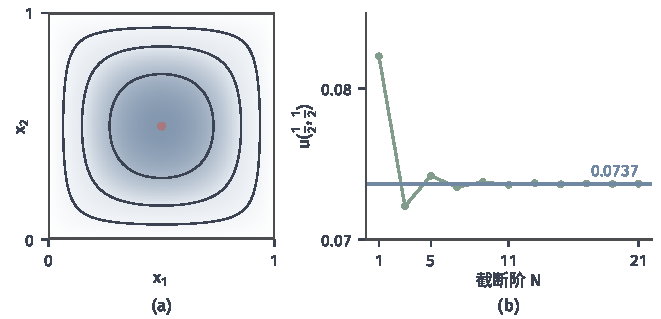
\includegraphics[width=112mm]{figures/06-differential-equations/02-partial-differential-equations/matplotlib/ellip-square-series/figure.pdf}
  \caption{单位正方形上$-\Delta u=1$、零Dirichlet边界的解。(a)$u$的取值，颜色越深值越大，等值线取$0.02,0.04,0.06$；角点附近的等值线被挤成圆角，红点是中心。(b)式~\eqref{eq:ellip-square-series}取$m,n\leq N$的中心值（绿）趋于蓝线。}
  \label{fig:ellip-square-series}
\end{BookInlineFigure}

\paragraph{零特征值}
把边界条件换成Neumann条件，特征问题的解变成$e_0=1$和$e_k=\sqrt2\cos(k\pi x)$，$\lambda_0=0$，$\lambda_k=k^2\pi^2$。式~\eqref{eq:ellip-spectral-solution}的第$k=0$项要除以$0$，不能直接用。

回到$\lambda_ku_k=f_k$这个关系，它对$k=0$说的是
\[
 0\cdot u_0=f_0=\int_0^1f\,\mathrm{d}x .
\]
这个等式有解当且仅当$f_0=0$，即相容条件~\eqref{eq:ellip-interval-compat}（$g_0=g_1=0$时）；一旦成立，$u_0$可以任取，这正是相差常数的不唯一。所以要先检查核空间上的分量，再对非零特征值做除法。

以$f=1-2x$为例，$f_0=0$，其余系数由分部积分算出，奇数$k$时$f_k=4\sqrt2/(k\pi)^2$，偶数$k$（$k\geq2$）时$f_k=0$。于是零均值的解是
\[
 u(x)=\sum_{k\ \text{奇}}\frac{8}{k^4\pi^4}\cos(k\pi x).
\]
在$x=0$处，第一项是$8/\pi^4\approx0.0821$，加上$k=3$的一项后约为$0.0831$，与前面的精确值$u(0)=1/12\approx0.0833$一致。


\section{弱形式}
\label{sec:ellip-weak}

前面的公式都假设解有连续的二阶导数。这个假设常常不成立。考虑一根由两种材料接成的棒：$a=1$于$(0,1/2)$，$a=4$于$(1/2,1)$，源项$f=1$，两端温度为零。系数在中点跳变，方程~\eqref{eq:ellip-1d-equation}中的$(au')'$在中点该怎么理解？

\paragraph{一个没有经典解的问题}
先按物理来算。热流$q=-au'$满足$q'=1$，所以$q(x)=x+C$在整段上是一条直线；热流穿过界面时不会凭空消失，因而$q$连续。由此得到$u'=-(x+C)/a$，它在中点有跳跃。

再用$u(0)=u(1)=0$定常数。温度沿整段的变化为零：
\[
 0=\int_0^1u'\,\mathrm{d}x=-\int_0^{1/2}(x+C)\,\mathrm{d}x-\frac14\int_{1/2}^1(x+C)\,\mathrm{d}x .
\]

算出两个积分并代入，得到
\[
 -\Bigl(\frac18+\frac C2\Bigr)-\frac14\Bigl(\frac38+\frac C2\Bigr)=-\frac7{32}-\frac{5C}8=0,
\]
所以$C=-7/20$。中点的温度是$u(1/2)=-(1/8+C/2)=1/20=0.05$。

图~\ref{fig:ellip-coefficient-jump}是这个解。$u$连续而在中点有折角，$u'$从$-0.15$跳到$-0.0375$，所以$u$不是$C^2$函数，甚至不是$C^1$函数，在中点逐点谈论方程是没有意义的。可是物理上这个解完全合理，热流$q$也是连续的。我们需要一种能接纳它的“解”的定义。

\begin{BookInlineFigure}
  \centering
  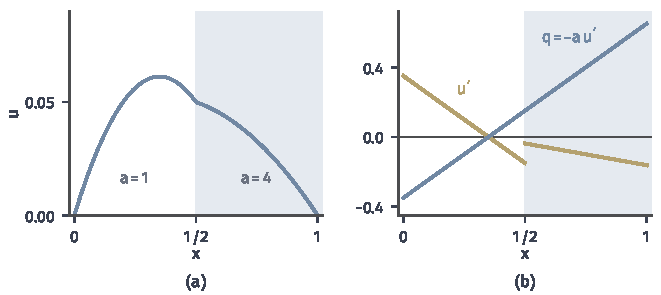
\includegraphics[width=112mm]{figures/06-differential-equations/02-partial-differential-equations/matplotlib/ellip-coefficient-jump/figure.pdf}
  \caption{两段材料接成的棒，$f=1$，两端温度为零，右半段（浅蓝底）导热率为$4$。(a)温度$u$连续，在中点有折角。(b)$u'$（黄）在中点跳跃，热流$q=-au'$（蓝）是一条连续的直线。}
  \label{fig:ellip-coefficient-jump}
\end{BookInlineFigure}

\paragraph{用测试函数检验}
经典解要求方程在每一点成立。换一种检验方式：取光滑的“探针”函数$v$，它只在某一小块区域内不为零，读取方程两边在这块区域上的加权平均。若对所有探针读数都相等，就说方程成立。这样的$v$称为\term{测试函数}（test function）。

用式~\eqref{eq:ellip-1d-equation}检验：两边乘以在两端为零的$v$，积分，并分部积分一次，把一个导数从$au'$移到$v$上：
\[
 \int_0^1fv\,\mathrm{d}x=-\int_0^1(au')'v\,\mathrm{d}x=\int_0^1au'v'\,\mathrm{d}x-\bigl[au'v\bigr]_0^1 .
\]
$v$在两端为零，边界项消失，于是
\begin{equation}
 \int_0^1a\,u'v'\,\mathrm{d}x=\int_0^1fv\,\mathrm{d}x .
 \label{eq:ellip-weak-1d}
\end{equation}

式~\eqref{eq:ellip-weak-1d}只含$u$的一阶导数，$a$也不需要可导。上面的折线型解可以直接代入。取$v=x(1-x)$，$v'=1-2x$，由$au'=-(x+C)$，两段合起来得到
\[
 \int_0^1au'v'\,\mathrm{d}x=-\int_0^1\Bigl(x-\frac7{20}\Bigr)(1-2x)\,\mathrm{d}x=\frac16,
\]
右端$\int_0^1fv\,\mathrm{d}x$也是$\int_0^1x(1-x)\,\mathrm{d}x=1/6$，两边相等。界面处的通量连续性不用单独写，它已经包含在弱形式中。

\begin{BookInlineFigure}
  \centering
  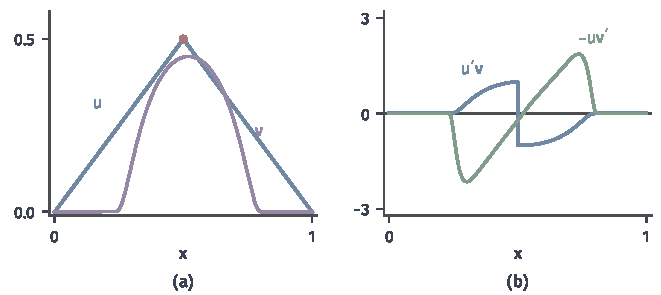
\includegraphics[width=112mm]{figures/06-differential-equations/02-partial-differential-equations/matplotlib/ellip-test-probe/figure.pdf}
  \caption{把导数转移到测试函数上。(a)$u=\tfrac12-\lvert x-\tfrac12\rvert$在红点处有折角，紫线是支撑在$(0.22,0.82)$内的光滑测试函数$v$（画为$0.45$倍）。(b)蓝线$u'v$在折角处跳跃，绿线$-uv'$连续。两条曲线不同，下方的积分却相同，数值积分都约为$-0.040$。}
  \label{fig:ellip-test-probe}
\end{BookInlineFigure}

这个动作的实质是让测试函数承担一半的导数，如图~\ref{fig:ellip-test-probe}所示。卷四用同样的动作定义了弱导数，这里只是把它用于方程。下面把多维的对应写出来，$\bm{A}$的条件沿用定义~\ref{def:ellip-uniform}。

\paragraph{多维的分部积分}
设$\Omega$是有界Lipschitz区域，$u,v$足够光滑。向量场$v\,\bm{A}\nabla u$的散度由乘积法则给出：
\[
 \nabla\cdot(v\bm{A}\nabla u)=\nabla v\cdot\bm{A}\nabla u+v\,\nabla\cdot(\bm{A}\nabla u) .
\]
对它用散度定理，得到
\begin{equation}
 \int_\Omega\bigl(-\nabla\cdot(\bm{A}\nabla u)\bigr)v\,\mathrm{d}\bm{x}
 =\int_\Omega\bm{A}\nabla u\cdot\nabla v\,\mathrm{d}\bm{x}-\int_{\partial\Omega}(\bm{n}\cdot\bm{A}\nabla u)\,v\,\mathrm{d}S .
 \label{eq:ellip-green-first}
\end{equation}
这是Green第一恒等式的一般形式。左端要两阶导数，右端的体积分只要一阶，边界项显示了边界通量在哪里出现。

由此定义贯穿全章的\term{双线性型}（bilinear form）
\begin{equation}
 a(u,v)=\int_\Omega\bm{A}\nabla u\cdot\nabla v\,\mathrm{d}\bm{x}.
 \label{eq:ellip-bilinear}
\end{equation}

\paragraph{用到的空间}
式~\eqref{eq:ellip-bilinear}有意义，只需要$u,v$有平方可积的一阶弱导数，这就是Sobolev空间$H^1(\Omega)$。回忆几个事实，其详细讨论可参考\BookChapterRef{chap:sobolev-spaces}{卷四第21章“Sobolev空间”}：

\begin{itemize}
 \item $H^1(\Omega)$由$L^2(\Omega)$中弱梯度也在$L^2$中的函数组成，按函数值和梯度的$L^2$内积之和定义内积后，它是Hilbert空间；
 \item 在有界Lipschitz区域上，存在把$H^1(\Omega)$映到$L^2(\partial\Omega)$的有界线性迹算子$\operatorname{Tr}$，对光滑到边界的函数就是限制到边界；
 \item $H^1_0(\Omega)$是$C_c^\infty(\Omega)$在$H^1$范数下的闭包，有界Lipschitz区域上它恰好是迹为零的函数组成的闭子空间。
\end{itemize}

本章记$\lVert v\rVert_2$为$L^2(\Omega)$范数，$\lVert\nabla v\rVert_2$为$\lVert\nabla v(\bm{x})\rVert_2$的$L^2(\Omega)$范数，$H^1$范数则由下式给出：
\[
 \lVert v\rVert_{H^1}^2=\lVert v\rVert_2^2+\lVert\nabla v\rVert_2^2 .
\]

函数值在边界上的约束要借助迹来表达，因为$H^1$函数只是几乎处处定义的等价类，边界是零测集，不能读取一个代表的边界值。右端的$\int_\Omega fv$只要求$f\in L^2(\Omega)$，甚至可以更弱：只要$v\mapsto\ell(v)$是$H^1_0(\Omega)$上的有界线性泛函。这样的泛函全体记为$H^{-1}(\Omega)$。

下面按边界条件的类型分别写出弱形式。两类条件的处理方式完全不同：一类写进函数空间，一类写进积分。

\subsection{Dirichlet条件}
\label{sec:ellip-weak-dirichlet}

对问题$-\nabla\cdot(\bm{A}\nabla u)=f$，$u=g$于$\partial\Omega$，式~\eqref{eq:ellip-green-first}中含未知的边界通量。测试函数取零迹时，这一项直接消失，所以测试函数应取在$H^1_0(\Omega)$中。

解要满足边界值$g$，这是对$u$的约束，写成$\operatorname{Tr}u=g$。要让这个条件有意义，$g$必须是某个$H^1(\Omega)$函数的迹，满足这个要求的边界函数组成迹空间，通常记为$H^{1/2}(\partial\Omega)$。于是有下面的定义。

\begin{definition}[Dirichlet问题的弱解]
\label{def:ellip-weak-dirichlet}
设$\Omega$是有界Lipschitz区域，$\bm{A}$一致椭圆，$f\in L^2(\Omega)$，$g=\operatorname{Tr}R$，其中$R\in H^1(\Omega)$。若$u\in H^1(\Omega)$满足$\operatorname{Tr}u=g$，且
\begin{equation}
 a(u,v)=\int_\Omega fv\,\mathrm{d}\bm{x}\qquad\text{对所有}\ v\in H^1_0(\Omega),
 \label{eq:ellip-weak-dirichlet}
\end{equation}
就称$u$是该问题的\term{弱解}（weak solution）。式~\eqref{eq:ellip-weak-dirichlet}称为\term{弱形式}（weak formulation）。
\end{definition}

这里要分清两组函数。候选的解称为试探函数，它们组成的集合是$\{u\in H^1(\Omega):\operatorname{Tr}u=g\}$，$g\neq0$时这不是线性空间，两个解之和的迹是$2g$。测试函数在$H^1_0(\Omega)$中，它是线性空间。

\paragraph{边界提升}
两者的关系是：试探函数的集合是$H^1_0(\Omega)$的一个平移。取任一满足$\operatorname{Tr}R=g$的函数$R$，称为$g$的\term{边界提升}（boundary lifting），令$w=u-R$，则$w\in H^1_0(\Omega)$。代入式~\eqref{eq:ellip-weak-dirichlet}，由$a$的双线性，问题化为
\begin{equation}
 a(w,v)=\int_\Omega fv\,\mathrm{d}\bm{x}-a(R,v)\qquad\text{对所有}\ v\in H^1_0(\Omega).
 \label{eq:ellip-lifted}
\end{equation}
边界数据的影响进入了右端的泛函，$w$在线性空间$H^1_0(\Omega)$中寻找，见图~\ref{fig:ellip-affine-trial}。

\begin{BookInlineFigure}
  \centering
  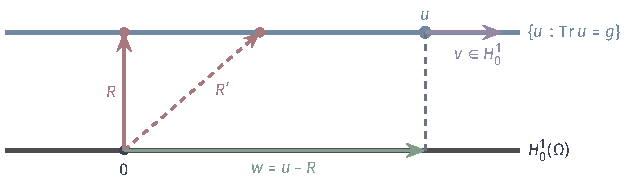
\includegraphics[width=110mm]{figures/06-differential-equations/02-partial-differential-equations/tikz/ellip-affine-trial/figure.pdf}
  \caption{试探集合与测试空间。深灰线是线性空间$H^1_0(\Omega)$，蓝线是平行的试探集合$\{u:\operatorname{Tr}u=g\}$，红色箭头是两个不同的提升$R$与$R'$。解$u$落在蓝线上，$w=u-R$（绿）在$H^1_0(\Omega)$中；试探集合内的移动方向（紫）都属于$H^1_0(\Omega)$，这就是测试函数取自$H^1_0(\Omega)$的原因。}
  \label{fig:ellip-affine-trial}
\end{BookInlineFigure}

提升不唯一，但$u$与提升的选择无关。回到例子$-u''=1$，$u(0)=1$，$u(1)=3$，解是$1+2x+x(1-x)/2$。取$R=1+2x$，得$w=x(1-x)/2$；取$R'=1+2x^2$，得$w'=5x(1-x)/2$。两个$w$不同，$R+w$与$R'+w'$却是同一个函数。

\paragraph{经典解与弱解}
新定义是否与原问题一致？经典解一定是弱解，反过来，足够光滑的弱解也是经典解，下面的定理说明了这一点。

\begin{theorem}[经典解与弱解]
\label{thm:ellip-classical-weak}
设$\Omega$是有界Lipschitz区域，$\bm{A}\in C^1(\overline\Omega)$一致椭圆，$f\in C(\overline\Omega)$，$u\in C^2(\overline\Omega)$，且在$\partial\Omega$上$u=g$。则$u$是弱解当且仅当
\begin{equation}
 -\nabla\cdot(\bm{A}\nabla u)=f\qquad\text{在}\ \Omega\ \text{内逐点成立}.
 \label{eq:ellip-classical}
\end{equation}
\end{theorem}

\begin{proof}
设$u$逐点满足方程。两边乘以$v\in C_c^\infty(\Omega)$，用式~\eqref{eq:ellip-green-first}，边界项为零，得到$a(u,v)=\int fv$。两边对$v$在$H^1$范数下都连续，$C_c^\infty(\Omega)$在$H^1_0(\Omega)$中稠密，所以等式对所有$v\in H^1_0(\Omega)$成立。

反过来，设$u$是弱解。对$v\in C_c^\infty(\Omega)$，式~\eqref{eq:ellip-weak-dirichlet}与式~\eqref{eq:ellip-green-first}合起来给出
\[
 \int_\Omega\bigl(-\nabla\cdot(\bm{A}\nabla u)-f\bigr)v\,\mathrm{d}\bm{x}=0 .
\]
括号内的函数连续。若它在某点不为零，就在该点附近保持同号，取在那里为正的局部凸起$v$，积分不为零，矛盾。所以它处处为零。
\end{proof}

用一个例子看弱形式怎样接纳更粗糙的数据。在$(0,1)$上固定$y$，令$\ell(v)=v(y)$，这是点源。$H^1_0(0,1)$的函数有连续代表，由Cauchy--Schwarz不等式，
\[
 \lvert v(y)\rvert=\Bigl\lvert\int_0^yv'\,\mathrm{d}x\Bigr\rvert\leq\sqrt y\,\lVert v'\rVert_2 ,
\]
所以$\ell$是有界泛函。Green函数$G(\cdot,y)$的斜率在$y$的左右分别是$1-y$和$-y$，代入弱形式，
\[
 \int_0^1G_x\,v'\,\mathrm{d}x=(1-y)\bigl(v(y)-v(0)\bigr)-y\bigl(v(1)-v(y)\bigr)=v(y),
\]
可见帐篷函数就是点源问题的弱解。

一维的这个例子不能推广到高维。$d\geq2$时$H^1$函数不必连续，点值不是有界泛函，点源的解$\Phi$的梯度也不平方可积，这一点在第~\ref{sec:ellip-lax-milgram}小节还会用到。

\subsection{Neumann与Robin条件}
\label{sec:ellip-weak-neumann}

若边界上规定的是通量，式~\eqref{eq:ellip-green-first}的边界项恰好是已知的量，这时不必再让它消失。

\paragraph{Neumann问题}
设$\bm{n}\cdot\bm{A}\nabla u=g$于$\partial\Omega$，$g\in L^2(\partial\Omega)$。两边乘以$v\in H^1(\Omega)$，用式~\eqref{eq:ellip-green-first}，把边界通量换成$g$，移到右端：
\begin{equation}
 a(u,v)=\int_\Omega fv\,\mathrm{d}\bm{x}+\int_{\partial\Omega}gv\,\mathrm{d}S\qquad\text{对所有}\ v\in H^1(\Omega),
 \label{eq:ellip-weak-neumann}
\end{equation}
其中边界积分里的$v$是迹。这里的试探函数和测试函数都在整个$H^1(\Omega)$中，空间没有施加任何边界约束。

\paragraph{Robin问题}
设$\bm{n}\cdot\bm{A}\nabla u+\beta u=g$，$\beta\geq0$。边界通量写成$g-\beta u$，代入后含未知函数$u$的边界项移到左端，得到
\begin{equation}
 a_\beta(u,v)=\int_\Omega fv\,\mathrm{d}\bm{x}+\int_{\partial\Omega}gv\,\mathrm{d}S\qquad\text{对所有}\ v\in H^1(\Omega),
 \label{eq:ellip-weak-robin}
\end{equation}
其中双线性型多了一个边界项：
\begin{equation}
 a_\beta(u,v)=a(u,v)+\int_{\partial\Omega}\beta uv\,\mathrm{d}S.
 \label{eq:ellip-robin-bilinear}
\end{equation}

\paragraph{边界条件怎样从积分中回来}
式~\eqref{eq:ellip-weak-neumann}没有明写边界条件，它是怎样被满足的？设弱解足够光滑。先取$v\in C_c^\infty(\Omega)$，边界项都消失，由定理~\ref{thm:ellip-classical-weak}的论证得到内部方程。

把内部方程代回，对一般的$v\in H^1(\Omega)$，式~\eqref{eq:ellip-green-first}给出
\[
 \int_{\partial\Omega}(\bm{n}\cdot\bm{A}\nabla u-g)\,v\,\mathrm{d}S=0 .
\]
$v$的边界值可以任意变动，所以$\bm{n}\cdot\bm{A}\nabla u=g$成立。这样由弱形式自动产生的条件称为\term{自然边界条件}（natural boundary condition）。对比之下，Dirichlet条件要事先放进试探集合，称为\term{本质边界条件}（essential boundary condition）。

用混合问题看这个机制的效果。方程$-u''=1$，$u(0)=0$，$u'(1)=0$，真解是$u_*=x-x^2/2$。弱形式是：$u$满足$u(0)=0$，且对所有$v(0)=0$的$v\in H^1(0,1)$有$\int_0^1u'v'\,\mathrm{d}x=\int_0^1v\,\mathrm{d}x$。

假如取一个满足内部方程但边界条件错误的候选$\tilde u=x(1-x)/2$，定义残量
\[
 R(v)=\int_0^1\tilde u'v'\,\mathrm{d}x-\int_0^1v\,\mathrm{d}x .
\]
分部积分，因$-\tilde u''=1$，积分项消去，只剩边界项：
\[
 R(v)=\bigl[\tilde u'v\bigr]_0^1=\tilde u'(1)\,v(1)=-\frac{v(1)}2 .
\]

图~\ref{fig:ellip-natural-residual}(b)画出这个关系。只要测试函数在$x=1$处不为零，$\tilde u$就通不过检验，而$u_*$对所有测试函数残量为零。例如$v=x$时，$\tilde u'v'=\tfrac12-x$的积分为$0$，$\int_0^1v=\tfrac12$，所以$R(v)=-\tfrac12$，与公式相符。

\begin{BookInlineFigure}
  \centering
  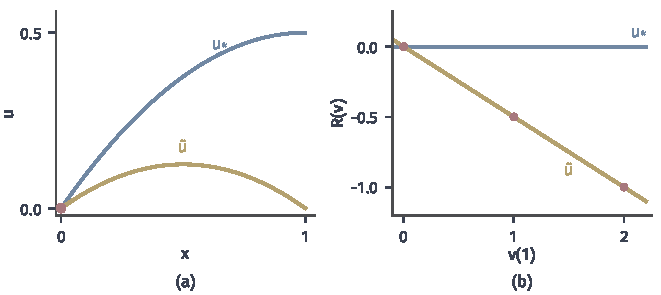
\includegraphics[width=112mm]{figures/06-differential-equations/02-partial-differential-equations/matplotlib/ellip-natural-residual/figure.pdf}
  \caption{自然边界条件由测试函数在边界上的自由度强制。(a)真解$u_*$（蓝）与错误候选$\tilde u$（黄），后者满足$u(1)=0$而不满足$u'(1)=0$。(b)残量$R(v)$随$v(1)$的变化，红点依次是$v=x(1-x)$、$v=x$或$x^2$、$v=2x$；$u_*$的残量恒为零。}
  \label{fig:ellip-natural-residual}
\end{BookInlineFigure}

把两类条件的对比列成表~\ref{tab:ellip-boundary-weak}。三种条件的差异只在于：边界的值由谁来负责。

\begin{BookInlineTable}
  \centering
  \caption{三类边界条件的弱形式。}
  \label{tab:ellip-boundary-weak}
  \begin{tabular}{llll}
    \toprule
    条件 & 试探函数 & 测试函数 & 边界数据的去向\\
    \midrule
    Dirichlet & $\operatorname{Tr}u=g$ & $H^1_0(\Omega)$ & 写进空间（本质）\\
    Neumann & $H^1(\Omega)$ & $H^1(\Omega)$ & 右端边界积分（自然）\\
    Robin & $H^1(\Omega)$ & $H^1(\Omega)$ & 左端$\beta$项与右端积分（自然）\\
    \bottomrule
  \end{tabular}
\end{BookInlineTable}


\section{存在、唯一与稳定性}
\label{sec:ellip-wellposed}

弱形式只是把问题重新写了一遍，解是否存在、是否唯一、是否连续依赖于数据，都还不知道。上一节的三种弱形式有共同的结构：在Hilbert空间$H$中求$u$，使得对所有$v\in H$有$a(u,v)=\ell(v)$。把这个抽象问题解决一次，再逐个边界条件检验假设。

\subsection{Lax--Milgram方法}
\label{sec:ellip-lax-milgram}

先看有限维。考虑方程组$\bm{A}\bm{x}=\bm{b}$，设存在$\alpha>0$，对所有$\bm{x}$有
\[
 \bm{x}^\top\bm{A}\bm{x}\geq\alpha\lVert\bm{x}\rVert_2^2 .
\]
这时矩阵一定可逆，因为$\bm{A}\bm{x}=\bm{0}$推出$\alpha\lVert\bm{x}\rVert_2^2\leq0$。这里不要求$\bm{A}$对称。

下面用一个非对称的矩阵核对：
\[
 \bm{A}=\begin{pmatrix}2&1\\-1&2\end{pmatrix},\qquad\bm{b}=\begin{pmatrix}3\\1\end{pmatrix}.
\]
二次型里的反对称部分互相抵消，$\bm{x}^\top\bm{A}\bm{x}=2\lVert\bm{x}\rVert_2^2$，所以$\alpha=2$。方程的解是$\bm{x}=(1,1)^\top$，并且
\[
 \lVert\bm{x}\rVert_2=\sqrt2\approx1.41\leq\frac{\lVert\bm{b}\rVert_2}{\alpha}=\frac{\sqrt{10}}2\approx1.58 .
\]

这个下界同时给出了可逆性和解的大小，无限维只需把三件事分别补上：把$a$变成算子，由下界得到单射与闭值域，再说明值域没有缺失的方向。第一件事要用Riesz表示定理：Hilbert空间上的每个有界线性泛函都能写成与唯一向量的内积，可参考\BookChapterRef{chap:linear-functionals}{卷四第16章“线性泛函”}。需要的条件如下。

\begin{definition}[有界与强制]
\label{def:ellip-bounded-coercive}
设$H$是实Hilbert空间，$a:H\times H\to\mathbb{R}$是双线性型。若存在$M>0$使
\begin{equation}
 \lvert a(u,v)\rvert\leq M\lVert u\rVert_H\lVert v\rVert_H\qquad\text{对所有}\ u,v\in H,
 \label{eq:ellip-bounded}
\end{equation}
就称$a$有界。若存在$\alpha>0$使
\begin{equation}
 a(v,v)\geq\alpha\lVert v\rVert_H^2\qquad\text{对所有}\ v\in H,
 \label{eq:ellip-coercive}
\end{equation}
就称$a$具有\term{强制性}（coercivity）。
\end{definition}

\begin{theorem}[Lax--Milgram定理]
\label{thm:ellip-lax-milgram}
设$H$是实Hilbert空间，$a$是$H$上有界且强制的双线性型，$\ell\in H^*$。则存在唯一的$u\in H$，使
\begin{equation}
 a(u,v)=\ell(v)\qquad\text{对所有}\ v\in H,
 \label{eq:ellip-abstract}
\end{equation}
并且
\begin{equation}
 \lVert u\rVert_H\leq\frac{\lVert\ell\rVert_{H^*}}{\alpha}.
 \label{eq:ellip-lm-estimate}
\end{equation}
\end{theorem}

\begin{proof}
\emph{第一步，化为算子方程。}由Riesz表示定理，对固定的$u$，$v\mapsto a(u,v)$是有界线性泛函，所以存在唯一的$Tu\in H$，使
\[
 a(u,v)=\langle Tu,v\rangle\qquad\text{对所有}\ v\in H .
\]
同样存在$h\in H$，使$\ell(v)=\langle h,v\rangle$，且$\lVert h\rVert_H=\lVert\ell\rVert_{H^*}$。由$a$的双线性，$T$线性。取$v=Tu$，式~\eqref{eq:ellip-bounded}给出$\lVert Tu\rVert_H\leq M\lVert u\rVert_H$，所以$T$有界。式~\eqref{eq:ellip-abstract}等价于$Tu=h$。

\emph{第二步，下界。}由强制性和Cauchy--Schwarz不等式，
\[
 \alpha\lVert v\rVert_H^2\leq a(v,v)=\langle Tv,v\rangle\leq\lVert Tv\rVert_H\lVert v\rVert_H .
\]
于是
\[
 \lVert Tv\rVert_H\geq\alpha\lVert v\rVert_H\qquad\text{对所有}\ v\in H .
\]
这说明$T$是单射。

\emph{第三步，值域闭。}设$Tv_n\to y$。对差$v_n-v_m$用下界，得到
\[
 \lVert v_n-v_m\rVert_H\leq\frac1\alpha\lVert Tv_n-Tv_m\rVert_H ,
\]
所以$(v_n)$是Cauchy列，收敛到某个$v$。$T$连续，得到$Tv=y$，所以$y$在值域中。

\emph{第四步，值域是全空间。}闭子空间的正交补为零时，子空间就是全空间。设$z$与值域正交。特别地，$z\perp Tz$，于是
\[
 \alpha\lVert z\rVert_H^2\leq a(z,z)=\langle Tz,z\rangle=0 ,
\]
所以$z=0$。因此$T$是双射，$u=T^{-1}h$是唯一的解。

\emph{第五步，估计。}在下界中取$v=u$，得到
\[
 \alpha\lVert u\rVert_H\leq\lVert Tu\rVert_H=\lVert h\rVert_H=\lVert\ell\rVert_{H^*} .
\]
\end{proof}

图~\ref{fig:ellip-lax-milgram}把第三、四步画了出来。下界保证蓝色的值域是闭的，不会缺少极限点；强制性保证与值域垂直的方向$z$不存在，因为若有这样的$z$，$Tz$也在值域中，与$z$垂直，就意味着$a(z,z)=0$。

\begin{BookInlineFigure}
  \centering
  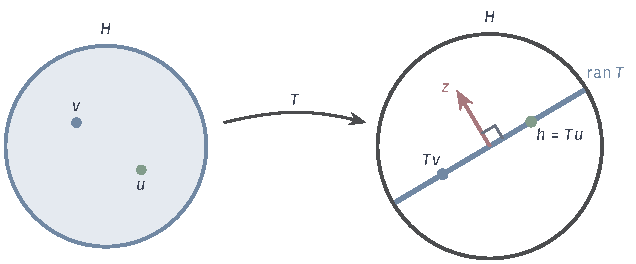
\includegraphics[width=108mm]{figures/06-differential-equations/02-partial-differential-equations/tikz/ellip-lax-milgram/figure.pdf}
  \caption{Lax--Milgram定理证明的几何图景。Riesz表示把$a$变成算子$T$，把$\ell$变成向量$h$，弱问题化为$Tu=h$。下界$\lVert Tv\rVert_H\geq\alpha\lVert v\rVert_H$使值域$\operatorname{ran}T$（蓝线）是闭子空间；红色的$z$若垂直于值域，强制性推出$z=0$，所以值域就是全空间。}
  \label{fig:ellip-lax-milgram}
\end{BookInlineFigure}

\paragraph{各条件的作用}
由式~\eqref{eq:ellip-lm-estimate}，数据之差$\ell_1-\ell_2$导致的解之差满足
\begin{equation}
 \lVert u_1-u_2\rVert_H\leq\frac{\lVert\ell_1-\ell_2\rVert_{H^*}}{\alpha}.
 \label{eq:ellip-lm-stability}
\end{equation}
所以弱问题适定：解存在、唯一，且连续依赖于右端。强制常数$\alpha$越小，同样的数据扰动带来的解的变化可能越大。

三个条件的分工很清楚。有界性让$T$有定义，而且是连续的。强制性同时负责单射、闭值域和满射。$\ell\in H^*$让右端能被表示成向量。

强制性是充分条件，不是必要条件。旋转矩阵$\begin{pmatrix}0&1\\-1&0\end{pmatrix}$可逆，却有$\bm{x}^\top\bm{A}\bm{x}=0$，定理不能用，但这只说明这条路走不通。而在具体方程中，强制性失败时往往确实出了问题：下面的Neumann问题就是这样。

$\ell$有界也不能省略。在$d=2$的单位圆盘上取点源，$\Phi$的梯度大小是$1/(2\pi r)$，能量积分
\[
 \int_{\lVert\bm{x}\rVert_2<1}\lVert\nabla\Phi\rVert_2^2\,\mathrm{d}\bm{x}=\int_0^1\frac{2\pi r}{4\pi^2r^2}\,\mathrm{d}r
\]
对数发散，所以点源问题的解不在$H^1$中。这与“点值不是$H^1_0$上的有界泛函”是同一件事的两面。

\subsection{Dirichlet问题}
\label{sec:ellip-dirichlet}

取$H=H^1_0(\Omega)$。式~\eqref{eq:ellip-uniform}的第二个条件和Cauchy--Schwarz不等式给出有界性：
\[
 \lvert a(u,v)\rvert\leq\kappa_{\max}\lVert\nabla u\rVert_2\lVert\nabla v\rVert_2 .
\]
强制性则要比较$\lVert\nabla v\rVert_2$与$\lVert v\rVert_{H^1}$。式~\eqref{eq:ellip-gradient-control}只控制了梯度，还需要用梯度控制函数本身。

这里需要的工具是Poincaré不等式，由卷四的结论，若$\Omega$有界，存在常数$C_P$，使
\begin{equation}
 \lVert v\rVert_2\leq C_P\lVert\nabla v\rVert_2\qquad\text{对所有}\ v\in H^1_0(\Omega).
 \label{eq:ellip-poincare}
\end{equation}
在$(0,1)$上最优常数是$1/\pi$，它在最低特征函数$\sin(\pi x)$上取到。这个不等式的含义是：函数在边界上被钉在零，要长高就必须爬坡，高度被坡度限制。

由式~\eqref{eq:ellip-poincare}，$\lVert\nabla v\rVert_2$在$H^1_0(\Omega)$上是与$H^1$范数等价的范数，因为
\[
 \lVert\nabla v\rVert_2^2\leq\lVert v\rVert_{H^1}^2\leq(1+C_P^2)\lVert\nabla v\rVert_2^2 .
\]
下面在$H^1_0(\Omega)$上取$\lVert v\rVert_{H^1_0}=\lVert\nabla v\rVert_2$，这时$\alpha=\kappa_{\min}$，$M=\kappa_{\max}$。

\begin{theorem}[Dirichlet问题的适定性]
\label{thm:ellip-dirichlet}
设$\Omega$是有界开集，$\bm{A}$一致椭圆，$f\in L^2(\Omega)$。则$-\nabla\cdot(\bm{A}\nabla u)=f$、零Dirichlet边界的弱解$u\in H^1_0(\Omega)$存在唯一，且
\begin{equation}
 \lVert\nabla u\rVert_2\leq\frac{C_P}{\kappa_{\min}}\lVert f\rVert_2 .
 \label{eq:ellip-dirichlet-estimate}
\end{equation}
若$\Omega$是有界Lipschitz区域，边界值$g=\operatorname{Tr}R$，$R\in H^1(\Omega)$，弱解同样存在唯一，且
\begin{equation}
 \lVert\nabla u\rVert_2\leq\frac{C_P}{\kappa_{\min}}\lVert f\rVert_2+\Bigl(1+\frac{\kappa_{\max}}{\kappa_{\min}}\Bigr)\lVert\nabla R\rVert_2 .
 \label{eq:ellip-dirichlet-inhom}
\end{equation}
\end{theorem}

\begin{proof}
先看$g=0$。令$\ell(v)=\int_\Omega fv\,\mathrm{d}\bm{x}$。由Cauchy--Schwarz不等式和式~\eqref{eq:ellip-poincare}，
\[
 \lvert\ell(v)\rvert\leq\lVert f\rVert_2\lVert v\rVert_2\leq C_P\lVert f\rVert_2\lVert\nabla v\rVert_2 ,
\]
所以$\lVert\ell\rVert\leq C_P\lVert f\rVert_2$。定理~\ref{thm:ellip-lax-milgram}给出唯一的解和估计式~\eqref{eq:ellip-dirichlet-estimate}。

再看一般的$g$。令$u=R+w$，$w$满足式~\eqref{eq:ellip-lifted}。其右端泛函满足
\[
 \Bigl\lvert\int_\Omega fv\,\mathrm{d}\bm{x}-a(R,v)\Bigr\rvert\leq\bigl(C_P\lVert f\rVert_2+\kappa_{\max}\lVert\nabla R\rVert_2\bigr)\lVert\nabla v\rVert_2 .
\]

定理~\ref{thm:ellip-lax-milgram}给出唯一的$w\in H^1_0(\Omega)$，且$\lVert\nabla w\rVert_2$不超过上式括号内的量除以$\kappa_{\min}$。对$u=R+w$用三角不等式，就得到式~\eqref{eq:ellip-dirichlet-inhom}。

唯一性：若$u_1,u_2$都是弱解，差$u_1-u_2\in H^1_0(\Omega)$满足齐次问题，由已证部分为零。
\end{proof}

式~\eqref{eq:ellip-dirichlet-inhom}说明解的大小由源项和边界提升共同决定，并且提升可以取$H^1$范数最小的那一个，于是估计实际上是对边界数据本身的。

用贯穿的例子核对。$\Omega=(0,1)$，$\kappa_{\min}=1$，$C_P=1/\pi$，$f=1$，$\lVert f\rVert_2=1$。解$u=x(1-x)/2$的导数是$1/2-x$，
\[
 \lVert u'\rVert_2=\Bigl(\int_0^1\bigl(\tfrac12-x\bigr)^2\,\mathrm{d}x\Bigr)^{1/2}=\frac1{\sqrt{12}}\approx0.289,
\]
而估计的上界是$1/\pi\approx0.318$，上界成立且相当紧。若取$f=\sin(\pi x)$，解是$\sin(\pi x)/\pi^2$，此时$\lVert u'\rVert_2=\lVert f\rVert_2/\pi$，估计取到等号，这说明常数$C_P/\kappa_{\min}$不能改进。

\paragraph{解算子与特征基}
第~\ref{sec:ellip-spectral}小节留下了一个问题：一般有界区域上，特征函数组成的基存在吗？弱解理论现在可以回答。设$\bm{A}$对称。定义解算子$S:L^2(\Omega)\to L^2(\Omega)$，$Sf$是源项为$f$的弱解。

由式~\eqref{eq:ellip-dirichlet-estimate}，$S$把$L^2$的有界集映为$H^1_0(\Omega)$的有界集。把$H^1_0(\Omega)$的函数零延拓到一个包含$\Omega$的球上，$H^1$有界集到$L^2$的紧嵌入就给出$S$是紧算子。一维时这一紧性更直接：$H^1(a,b)$的有界集由Sobolev不等式一致有界、等度Hölder连续，由Arzelà--Ascoli定理在$C[a,b]$中相对紧，从而在$L^2(a,b)$中相对紧。

$S$还是自伴的。记$u=Sf$，$w=Sh$，把它们互相作为测试函数，由弱形式和$a$的对称性，
\[
 \langle h,Sf\rangle=a(w,u)=a(u,w)=\langle f,Sh\rangle .
\]
$S$也是正的，且是单射，因为$f\neq0$时$u\neq0$，从而$\langle f,Sf\rangle=a(u,u)>0$。

由紧自伴算子的谱定理（可参考\BookChapterRef{chap:operator-spectra}{卷四第18章“算子谱”}），存在$L^2(\Omega)$的标准正交基$(e_k)$，使$Se_k=\mu_ke_k$，$\mu_k>0$，$\mu_k\to0$。令$\lambda_k=1/\mu_k$，则$\lambda_k\to\infty$，$e_k\in H^1_0(\Omega)$，且
\[
 a(e_k,v)=\lambda_k\langle e_k,v\rangle\qquad\text{对所有}\ v\in H^1_0(\Omega) .
\]
这就是特征问题~\eqref{eq:ellip-eigenproblem}的弱形式，而$Sf=\sum_k\mu_kf_ke_k$正是式~\eqref{eq:ellip-spectral-solution}。

\subsection{Neumann问题}
\label{sec:ellip-neumann}

在式~\eqref{eq:ellip-weak-neumann}中取$v=1$，$\nabla v=0$，左端为零，得到
\begin{equation}
 \int_\Omega f\,\mathrm{d}\bm{x}+\int_{\partial\Omega}g\,\mathrm{d}S=0.
 \label{eq:ellip-neumann-compat}
\end{equation}
这是相容条件~\eqref{eq:ellip-interval-compat}的多维形式，意义仍是总量收支为零。不满足这个条件，弱解就不存在。

反过来，$a$在$H^1(\Omega)$上不强制：常数函数$v=1$满足$a(v,v)=0$。若$\Omega$连通，$a(v,v)=0$蕴含$\nabla v=0$，$v$是常数，所以核空间恰好是常数。若$\Omega$不连通，每个连通分支上都可以独立取常数，核空间更大，相容条件也要逐分支成立。

这与奇异矩阵的情形完全相同。图~\ref{fig:ellip-energy-valley}用两个未知量的二次函数$\frac12\bm{c}^\top\bm{K}\bm{c}-\bm{b}^\top\bm{c}$比较三种情形，其极小点满足$\bm{K}\bm{c}=\bm{b}$。(a)是正定的$\bm{K}$，等高线是椭圆，有唯一的极小点。(b)的$\bm{K}=\begin{pmatrix}1&-1\\-1&1\end{pmatrix}$有核方向$(1,1)^\top$，$\bm{b}$与核方向正交时，极小点组成一条线。(c)的$\bm{b}$不与核方向正交，函数沿核方向一直下降，没有极小点。

\begin{BookInlineFigure}
  \centering
  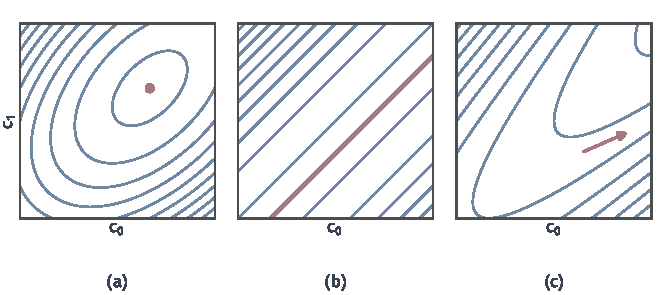
\includegraphics[width=112mm]{figures/06-differential-equations/02-partial-differential-equations/matplotlib/ellip-energy-valley/figure.pdf}
  \caption{核空间的有限维图景，蓝线是$\frac12\bm{c}^\top\bm{K}\bm{c}-\bm{b}^\top\bm{c}$的等高线。(a)$\bm{K}$的对角元为$2$、非对角元为$-1$，$\bm{b}=(1,1)^\top$，唯一极小点$(1,1)$（红）。(b)$\bm{K}$奇异，$\bm{b}=(1,-1)^\top$与核方向$(1,1)^\top$正交，极小点是红线$c_0-c_1=1$。(c)同样的$\bm{K}$，$\bm{b}=(1,0)^\top$，沿红色箭头方向函数无下界。}
  \label{fig:ellip-energy-valley}
\end{BookInlineFigure}

处理办法是先去掉核方向。取零均值子空间
\begin{equation}
 V=\Bigl\{v\in H^1(\Omega):\int_\Omega v\,\mathrm{d}\bm{x}=0\Bigr\}.
 \label{eq:ellip-zero-mean}
\end{equation}
由卷四的零均值Poincaré不等式，在有界连通Lipschitz区域上存在$C_W$，使$\lVert v\rVert_2\leq C_W\lVert\nabla v\rVert_2$对$v\in V$成立。于是$\lVert\nabla\cdot\rVert_2$是$V$上的等价范数，$a$在$V$上强制，$\alpha=\kappa_{\min}$。

迹算子有界，再用上面的等价范数，就存在常数$C_\partial$，使
\begin{equation}
 \lVert\operatorname{Tr}v\rVert_{L^2(\partial\Omega)}\leq C_\partial\lVert\nabla v\rVert_2\qquad\text{对所有}\ v\in V.
 \label{eq:ellip-trace-zero-mean}
\end{equation}

\begin{theorem}[Neumann问题的适定性]
\label{thm:ellip-neumann}
设$\Omega$是有界连通Lipschitz区域，$\bm{A}$一致椭圆，$f\in L^2(\Omega)$，$g\in L^2(\partial\Omega)$。式~\eqref{eq:ellip-weak-neumann}有解当且仅当式~\eqref{eq:ellip-neumann-compat}成立。此时解在相差一个常数的意义下唯一，零均值的解$u\in V$满足
\begin{equation}
 \lVert\nabla u\rVert_2\leq\frac1{\kappa_{\min}}\bigl(C_W\lVert f\rVert_2+C_\partial\lVert g\rVert_{L^2(\partial\Omega)}\bigr).
 \label{eq:ellip-neumann-estimate}
\end{equation}
\end{theorem}

\begin{proof}
必要性已经证明。设相容条件成立，令$\ell(v)=\int_\Omega fv+\int_{\partial\Omega}gv$。在$V$上，由Cauchy--Schwarz不等式和式~\eqref{eq:ellip-trace-zero-mean}，
\[
 \lvert\ell(v)\rvert\leq\bigl(C_W\lVert f\rVert_2+C_\partial\lVert g\rVert_{L^2(\partial\Omega)}\bigr)\lVert\nabla v\rVert_2 .
\]
定理~\ref{thm:ellip-lax-milgram}给出唯一的$u\in V$和估计式~\eqref{eq:ellip-neumann-estimate}，它对所有$v\in V$满足$a(u,v)=\ell(v)$。

还要把测试函数从$V$扩大到$H^1(\Omega)$。任取$v\in H^1(\Omega)$，令$\bar v=\lvert\Omega\rvert^{-1}\int_\Omega v$，则$v-\bar v\in V$。$a(u,\bar v)=0$，因为常数的梯度为零；$\ell(\bar v)=0$，因为相容条件成立。于是
\[
 a(u,v)=a(u,v-\bar v)=\ell(v-\bar v)=\ell(v) .
\]

若$u_1,u_2$都是解，差$z=u_1-u_2$满足$a(z,z)=0$，由式~\eqref{eq:ellip-gradient-control}，$\nabla z=0$，$\Omega$连通，故$z$是常数。
\end{proof}

用前面的例子核对。$\Omega=(0,1)$，$f=1-2x$，$C_W=1/\pi$，$\lVert f\rVert_2=1/\sqrt3$。解的导数$u'=x^2-x$，
\[
 \lVert u'\rVert_2=\Bigl(\int_0^1(x^2-x)^2\,\mathrm{d}x\Bigr)^{1/2}=\frac1{\sqrt{30}}\approx0.183,
\]
上界$C_W\lVert f\rVert_2=1/(\pi\sqrt3)\approx0.184$，几乎取到等号，因为$f$很接近第一个非常数的特征函数。

这里的估计式~\eqref{eq:ellip-neumann-estimate}只对零均值的代表成立，也只能如此：加上常数后，解可以任意大，却仍是解。

\subsection{Robin问题}
\label{sec:ellip-robin}

Robin问题的$a_\beta$比$a$多了边界项$\int_{\partial\Omega}\beta v^2$。常数函数在$a$中的能量为零，在这里要付出边界代价。边界项能否像Poincaré不等式那样补足对函数本身的控制？

先看一个可以直接解的例子。在$(0,1)$上取$-u''=1$，两端都是$\bm{n}\cdot\nabla u+\beta u=0$，$\beta>0$。由对称性，解形如$x(1-x)/2+c$，代入左端条件：
\[
 -u'(0)+\beta u(0)=-\frac12+\beta c=0 ,
\]
所以
\begin{equation}
 u(x)=\frac{x(1-x)}2+\frac1{2\beta}.
 \label{eq:ellip-robin-example}
\end{equation}

图~\ref{fig:ellip-robin-beta}显示$\beta$的作用。$\beta\to\infty$时，边界换热无限快，解收敛到Dirichlet问题的解。$\beta\to0$时，$u$的常数部分$1/(2\beta)$趋于无穷，解的范数爆炸；极限的Neumann问题$f=1$本来就不相容。收支也是平衡的：总产热$1$经两端散出，$\beta(u(0)+u(1))=1$。

\begin{BookInlineFigure}
  \centering
  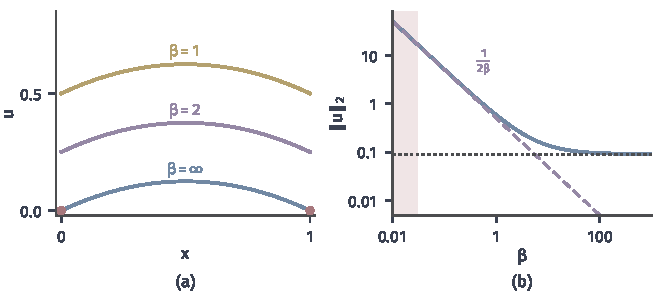
\includegraphics[width=112mm]{figures/06-differential-equations/02-partial-differential-equations/matplotlib/ellip-robin-beta/figure.pdf}
  \caption{$-u''=1$、两端Robin条件的解。(a)$\beta=1,2$时（黄、紫）解被整体抬高$1/(2\beta)$，$\beta\to\infty$时趋于蓝线的Dirichlet解。(b)$\lVert u\rVert_2$随$\beta$的变化：$\beta\to0$时沿紫色虚线$1/(2\beta)$爆炸（红底区域接近不相容的Neumann极限），$\beta\to\infty$时趋于点线$1/\sqrt{120}$。}
  \label{fig:ellip-robin-beta}
\end{BookInlineFigure}

这个例子说明，强制常数必然随$\beta$退化，所以需要一条统一的不等式，把$\beta$的作用写进去。

\begin{lemma}[边界项给出的Poincaré不等式]
\label{lem:ellip-robin-poincare}
设$\Omega$是有界连通Lipschitz区域，$\beta\in L^\infty(\partial\Omega)$，$\beta\geq0$，$\int_{\partial\Omega}\beta\,\mathrm{d}S>0$。则存在常数$C_R$，使
\begin{equation}
 \lVert v\rVert_2^2\leq C_R\Bigl(\lVert\nabla v\rVert_2^2+\int_{\partial\Omega}\beta v^2\,\mathrm{d}S\Bigr)\qquad\text{对所有}\ v\in H^1(\Omega).
 \label{eq:ellip-robin-poincare}
\end{equation}
\end{lemma}

\begin{proof}
用反证法。若不等式不成立，存在序列$(v_n)\subset H^1(\Omega)$，$\lVert v_n\rVert_2=1$，并且
\[
 \lVert\nabla v_n\rVert_2^2+\int_{\partial\Omega}\beta v_n^2\,\mathrm{d}S\to0 .
\]
序列在$H^1$中有界，由$H^1(\Omega)$到$L^2(\Omega)$的紧嵌入，有子列在$L^2(\Omega)$中收敛到某个$v$，$\lVert v\rVert_2=1$。子列的梯度趋于零，所以子列在$H^1$中也是Cauchy列，收敛到$v$，且$\nabla v=0$。

$\Omega$连通，所以$v$等于常数$c$，由$\lVert v\rVert_2=1$知$c\neq0$。迹算子连续，$\operatorname{Tr}v_n\to c$于$L^2(\partial\Omega)$，$\beta$有界，于是
\[
 \int_{\partial\Omega}\beta v_n^2\,\mathrm{d}S\to c^2\int_{\partial\Omega}\beta\,\mathrm{d}S>0 ,
\]
这与假设矛盾。
\end{proof}

这个证明用了紧嵌入，所以常数$C_R$是非构造性的。证明的核心很直白：能让所有控制量都趋于零的只有常数，而边界上正的$\beta$排除了常数。

\begin{theorem}[Robin问题的适定性]
\label{thm:ellip-robin}
设$\Omega$是有界连通Lipschitz区域，$\bm{A}$一致椭圆，$\beta$满足引理~\ref{lem:ellip-robin-poincare}的条件，$f\in L^2(\Omega)$，$g\in L^2(\partial\Omega)$。则式~\eqref{eq:ellip-weak-robin}存在唯一的解$u\in H^1(\Omega)$，且存在只依赖于$\Omega,\bm{A},\beta$的常数$C$，使
\begin{equation}
 \lVert u\rVert_{H^1}\leq C\bigl(\lVert f\rVert_2+\lVert g\rVert_{L^2(\partial\Omega)}\bigr).
 \label{eq:ellip-robin-estimate}
\end{equation}
\end{theorem}

\begin{proof}
由迹定理，存在$C_{\mathrm{Tr}}$，使
\[
 \lVert\operatorname{Tr}v\rVert_{L^2(\partial\Omega)}\leq C_{\mathrm{Tr}}\lVert v\rVert_{H^1} .
\]
于是$a_\beta$有界：
\[
 \lvert a_\beta(u,v)\rvert\leq\bigl(\kappa_{\max}+\lVert\beta\rVert_\infty C_{\mathrm{Tr}}^2\bigr)\lVert u\rVert_{H^1}\lVert v\rVert_{H^1} .
\]
右端泛函也有界，其范数不超过$\lVert f\rVert_2+C_{\mathrm{Tr}}\lVert g\rVert_{L^2(\partial\Omega)}$。

由式~\eqref{eq:ellip-gradient-control}，令$\kappa_0=\min(\kappa_{\min},1)$，
\[
 a_\beta(v,v)\geq\kappa_0\Bigl(\lVert\nabla v\rVert_2^2+\int_{\partial\Omega}\beta v^2\,\mathrm{d}S\Bigr) .
\]
由式~\eqref{eq:ellip-robin-poincare}，
\[
 \lVert v\rVert_{H^1}^2\leq(1+C_R)\Bigl(\lVert\nabla v\rVert_2^2+\int_{\partial\Omega}\beta v^2\,\mathrm{d}S\Bigr) .
\]
所以$a_\beta$强制，$\alpha=\kappa_0/(1+C_R)$。定理~\ref{thm:ellip-lax-milgram}给出结论。
\end{proof}

条件$\int_{\partial\Omega}\beta>0$不能去掉。$\beta\equiv0$时问题退回Neumann问题，核空间是常数，唯一性丢失。条件$\beta\geq0$也不能随意放宽。在$(0,1)$上取两端$\beta=-2$，考察$-u''=0$，函数$u=1-2x$满足
\[
 -u'(0)+\beta u(0)=2-2=0,\qquad u'(1)+\beta u(1)=-2+2=0 ,
\]
这是一个非零的解，所以齐次问题不唯一。负的$\beta$相当于边界不断向棒内放热，且放热量随温度增长，边界项不再贡献能量，而是削弱能量。

三类边界条件的结论可以这样总结：Dirichlet问题靠零迹排除常数，Robin问题靠边界代价排除常数，Neumann问题排除不了常数，只能把常数方向分离出去，并要求数据与之相容。


\section{能量极小}
\label{sec:ellip-energy}

一根绷紧的弦受到载荷后停在某个形状，这个形状是所有可能形状中总势能最小的。Poisson方程的弱解是否也是某种能量的极小点？第~\ref{sec:ellip-wellposed}节的三种弱形式都能这样解释吗？

\paragraph{能量泛函}
对$H$上的双线性型$a$和右端泛函$\ell$，定义二次泛函
\begin{equation}
 J(v)=\frac12a(v,v)-\ell(v).
 \label{eq:ellip-energy}
\end{equation}
对Dirichlet问题，$a$和$\ell$分别是式~\eqref{eq:ellip-bilinear}与$\int_\Omega fv$，所以
\[
 J(v)=\frac12\int_\Omega\bm{A}\nabla v\cdot\nabla v\,\mathrm{d}\bm{x}-\int_\Omega fv\,\mathrm{d}\bm{x} .
\]
第一项是梯度的储能，第二项是载荷做功的相反数，两者折中，形成平衡。

有限维的类比是对称正定的$\bm{K}$和二次函数$\frac12\bm{c}^\top\bm{K}\bm{c}-\bm{b}^\top\bm{c}$，令梯度为零，正是$\bm{K}\bm{c}=\bm{b}$。下面的定理是这件事的无限维版本。泛函的方向导数与极小点的一般理论可参考\BookChapterRef{chap:functional-optimization-variation}{卷五第29章“泛函优化”}，这里的二次泛函可以直接展开，不需要一般理论。

\begin{theorem}[弱解是能量的唯一极小点]
\label{thm:ellip-energy}
设$H$是实Hilbert空间，$a$是$H$上有界、强制且对称的双线性型，$\ell\in H^*$。对$u\in H$，下面两条等价：
\begin{enumerate}
 \item $a(u,v)=\ell(v)$对所有$v\in H$成立；
 \item $u$是$J$在$H$上的极小点。
\end{enumerate}
极小点存在且唯一，并且对所有$w\in H$，
\begin{equation}
 J(u+w)-J(u)=\frac12a(w,w).
 \label{eq:ellip-energy-gap}
\end{equation}
\end{theorem}

\begin{proof}
对任意$u,w\in H$，由双线性与对称性展开，
\[
 J(u+w)=J(u)+\bigl(a(u,w)-\ell(w)\bigr)+\frac12a(w,w).
\]

设第1条成立，括号为零，就得到式~\eqref{eq:ellip-energy-gap}。由强制性，$w\neq0$时$a(w,w)>0$，所以$u$是唯一的极小点。

设第2条成立。任取$v\in H$和实数$t$，取$w=tv$，极小性给出
\[
 0\leq J(u+tv)-J(u)=t\bigl(a(u,v)-\ell(v)\bigr)+\frac{t^2}2a(v,v).
\]
右端是$t$的二次函数，在$t=0$处取最小值$0$，所以一次项系数为零，即第1条成立。

极小点的存在由定理~\ref{thm:ellip-lax-milgram}给出。
\end{proof}

式~\eqref{eq:ellip-energy-gap}比“极小”的说法更强：任何候选的能量超出最优能量的部分，恰好是它到解的距离在能量范数下的平方的一半。

对称情形下，存在性也可以不用Lax--Milgram定理。此时$a(\cdot,\cdot)$本身是$H$上的一个等价内积，Riesz表示定理直接给出解；或者取极小化序列用平行四边形恒等式证明它是Cauchy列。这是对称问题的简化，非对称问题走不通。

\paragraph{手算比较}
继续用$-u''=1$，$u(0)=u(1)=0$，这时$J(v)=\frac12\int_0^1v'^2-\int_0^1v$。把真解$u_*=x(1-x)/2$代入：
\[
 J(u_*)=\frac12\cdot\frac1{12}-\frac1{12}=-\frac1{24}\approx-0.04167 .
\]

取几个其他的候选比较，都先把幅度调到各自的最优值。形如$cx(1-x)$的候选有
\[
 J=\frac{c^2}6-\frac c6,
\]
它在$c=1/2$处最小，正好回到真解。帐篷函数$s\min(x,1-x)$有$J=s^2/2-s/4$，最优幅度$s=1/4$给出$J=-1/32\approx-0.03125$。单个正弦$c\sin(\pi x)$的最优幅度是$c=4/\pi^3$，给出$J=-4/\pi^4\approx-0.04106$。

\begin{BookInlineFigure}
  \centering
  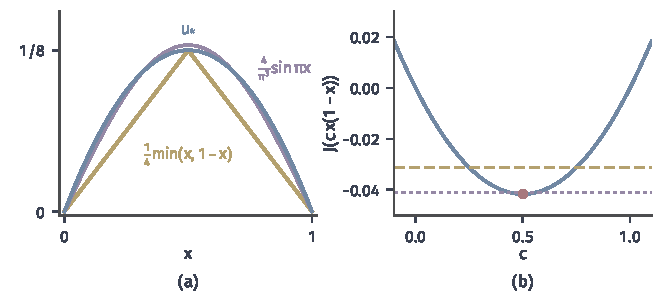
\includegraphics[width=112mm]{figures/06-differential-equations/02-partial-differential-equations/matplotlib/ellip-energy-competition/figure.pdf}
  \caption{能量比较，$f=1$，零边界。(a)真解$u_*$（蓝）与两个候选：帐篷（黄）和单个正弦（紫）。(b)蓝线是$J(cx(1-x))$，红点是$c=1/2$处的最小值$-1/24$；黄色虚线和紫色点线分别是帐篷和正弦的能量，都高于$-1/24$。}
  \label{fig:ellip-energy-competition}
\end{BookInlineFigure}

图~\ref{fig:ellip-energy-competition}表明，正弦候选的形状已经非常接近真解，能量也只比最优高$0.0006$。式~\eqref{eq:ellip-energy-gap}解释了能量如此接近的原因：能量差是误差的平方，误差小时，能量差更小。

\paragraph{边界条件的归宿}
能量泛函还给出了本质边界条件与自然边界条件的另一种解释。Dirichlet问题的约束是对可行集的限制，要在集合$\{v\in H^1(\Omega):\operatorname{Tr}v=g\}$上极小化。Neumann问题没有约束，$J$里多一项$-\int_{\partial\Omega}gv$，边界条件是极小性自己产生的。Robin问题里，$\frac12\int_{\partial\Omega}\beta v^2$是边界代价，$\beta\to\infty$时迫使$v$在边界上趋于零，这正是图~\ref{fig:ellip-robin-beta}看到的极限。

Neumann问题的能量沿常数方向是平的，这就是图~\ref{fig:ellip-energy-valley}的情形：相容条件成立时极小点组成一条直线，不成立时能量沿常数方向无下界，极小点不存在。

\paragraph{非对称问题}
对称性不能省去。考虑带一阶项的方程$-u''+bu'=f$，$u(0)=u(1)=0$，$b$是常数。在$H^1_0(0,1)$上，弱形式的双线性型是
\begin{equation}
 a_b(u,v)=\int_0^1u'v'\,\mathrm{d}x+b\int_0^1u'v\,\mathrm{d}x .
 \label{eq:ellip-convection-form}
\end{equation}

它有界，因为由Poincaré不等式，
\[
 \Bigl\lvert b\int_0^1u'v\,\mathrm{d}x\Bigr\rvert\leq\lvert b\rvert\lVert u'\rVert_2\lVert v\rVert_2\leq\frac{\lvert b\rvert}\pi\lVert u'\rVert_2\lVert v'\rVert_2 .
\]
它也强制，而且强制常数与$b$无关：
\[
 \int_0^1v'v\,\mathrm{d}x=\frac12\bigl[v^2\bigr]_0^1=0,\qquad\text{所以}\quad a_b(v,v)=\lVert v'\rVert_2^2 .
\]
由Lax--Milgram定理，弱解存在唯一。$f=1$时可以解出
\begin{equation}
 u_b(x)=\frac xb-\frac{\mathrm{e}^{bx}-1}{b(\mathrm{e}^b-1)},\qquad b\neq0 .
 \label{eq:ellip-convection-solution}
\end{equation}

这个解不是$J(v)=\frac12a_b(v,v)-\ell(v)$的极小点。由上式，$\frac12a_b(v,v)=\frac12\lVert v'\rVert_2^2$，$b$根本没有出现在$J$中。$J$的极小点对每个$b$都是$b=0$的解$x(1-x)/2$，而图~\ref{fig:ellip-nonsymmetric}中真正的解随$b$的增大明显向右偏移。

一般地，$J$在$u$处沿$w$的变化率是$\frac12(a(u,w)+a(w,u))-\ell(w)$，只看到$a$的对称部分。

\begin{BookInlineFigure}
  \centering
  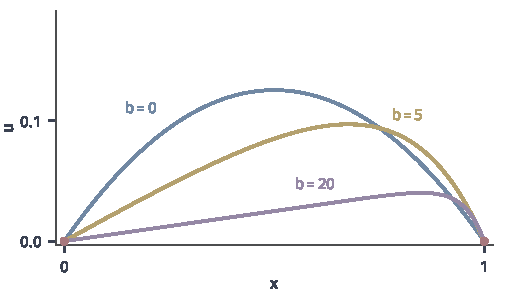
\includegraphics[width=86mm]{figures/06-differential-equations/02-partial-differential-equations/matplotlib/ellip-nonsymmetric/figure.pdf}
  \caption{非对称问题$-u''+bu'=1$的解随$b$的变化。$b=0$（蓝）时对称，$b=5$（黄）与$b=20$（紫）时被对流推向右端，在$x=1$附近形成边界层。双线性型的二次部分与$b$无关，所以这些解不能由式~\eqref{eq:ellip-energy}的极小化得到。}
  \label{fig:ellip-nonsymmetric}
\end{BookInlineFigure}

区间上的这个例子还可以用积分因子补救。在方程两边乘以$\mathrm{e}^{-bx}$，得到$-(\mathrm{e}^{-bx}u')'=\mathrm{e}^{-bx}f$，它在带权的能量下又是对称的。多维情形中，只有当一阶项的系数是某个函数的梯度时，这种办法才能奏效，否则一般不存在把问题化成能量极小的权函数。所以结论是：Lax--Milgram定理适用的范围比能量极小更广，能量极小只是对称情形的额外结构。


\section{最大值原理}
\label{sec:ellip-maximum}

前面的能量估计控制的是平方积分的大小，没有告诉我们解在哪里最大。温度分布有一个直观的事实：没有内部热源时，最高温只能出现在边界上。若内部出现了一个比周围都热的点，热量就会从它流向四周，无法平衡。把这个直觉变成定理，需要用到方程的符号结构。

\paragraph{调和函数是平均值}
上面的直觉有一个精确的版本：调和函数在每一点的值，等于以该点为心的任意球面上的平均值，这称为\term{平均值性质}（mean value property）。

\begin{theorem}[平均值性质]
\label{thm:ellip-mean-value}
设$u\in C^2(\Omega)$在$\Omega$内调和，$\overline{B_r(\bm{x})}\subset\Omega$。则
\begin{equation}
 u(\bm{x})=\frac1{\lvert\partial B_r\rvert}\int_{\partial B_r(\bm{x})}u\,\mathrm{d}S,
 \label{eq:ellip-mean-value}
\end{equation}
并且对球体上的平均，同样的等式成立。
\end{theorem}

\begin{proof}
把球面积分写成单位球面$S$上的平均，令
\[
 m(r)=\frac1{\lvert S\rvert}\int_Su(\bm{x}+r\bm{\omega})\,\mathrm{d}\sigma(\bm{\omega}) .
\]
对$r$求导，换回半径$r$的球面，并用散度定理：
\[
 m'(r)=\frac1{\lvert\partial B_r\rvert}\int_{\partial B_r}\partial_{\bm{n}}u\,\mathrm{d}S=\frac1{\lvert\partial B_r\rvert}\int_{B_r}\Delta u\,\mathrm{d}\bm{y}=0 .
\]
所以$m$是常数，又因$u$连续，$r\to0$时$m(r)\to u(\bm{x})$。这就证明了式~\eqref{eq:ellip-mean-value}。球体上的平均是不同半径的球面平均对$r$的加权积分，也等于$u(\bm{x})$。
\end{proof}

图~\ref{fig:ellip-harmonic-saddle}中，$u=x_1^2-x_2^2$在圆盘上调和。圆周上的值有高有低，平均后恰好是圆心的值。这个函数的最大值出现在边界上的两个红点，最小值在两个紫点，内部的鞍点不是极值。

\begin{BookInlineFigure}
  \centering
  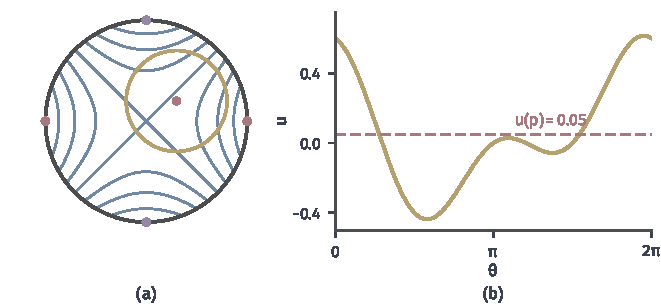
\includegraphics[width=112mm]{figures/06-differential-equations/02-partial-differential-equations/matplotlib/ellip-harmonic-saddle/figure.pdf}
  \caption{调和函数$u=x_1^2-x_2^2$。(a)单位圆盘内的等值线，红点是边界上的最大值点，紫点是最小值点。黄圆心在$\bm{p}=(0.3,0.2)$，半径$0.5$。(b)黄圆上$u$的取值（黄），红色虚线是圆心值$u(\bm{p})=0.05$，也是这些取值的平均值。}
  \label{fig:ellip-harmonic-saddle}
\end{BookInlineFigure}

\paragraph{Laplace算子的最大值原理}
把“内部的值不超过边界上的值”写成定理，就是\term{最大值原理}（maximum principle）。它只要求$-\Delta u\leq0$，即区域内部没有热源，但可以有热汇。

\begin{theorem}[弱最大值原理]
\label{thm:ellip-weak-max}
设$\Omega$是有界开集，$u\in C^2(\Omega)\cap C(\overline\Omega)$，在$\Omega$内$-\Delta u\leq0$。则
\begin{equation}
 \max_{\overline\Omega}u=\max_{\partial\Omega}u.
 \label{eq:ellip-weak-max}
\end{equation}
\end{theorem}

\begin{proof}
先处理严格的情形。若$-\Delta v<0$，$v$不可能在内部取最大值：在内部最大值点，每个方向的二阶导数都不超过零，$\Delta v\leq0$，与$\Delta v>0$矛盾。

对一般的$u$，令$v_\varepsilon=u+\varepsilon\lVert\bm{x}\rVert_2^2$，$\varepsilon>0$。则$\Delta v_\varepsilon=\Delta u+2d\varepsilon>0$，所以$v_\varepsilon$的最大值在边界上取得，于是
\[
 \max_{\overline\Omega}u\leq\max_{\overline\Omega}v_\varepsilon=\max_{\partial\Omega}v_\varepsilon\leq\max_{\partial\Omega}u+\varepsilon\max_{\partial\Omega}\lVert\bm{x}\rVert_2^2 .
\]
令$\varepsilon\to0$，得到$\max_{\overline\Omega}u\leq\max_{\partial\Omega}u$。反向不等式由$\partial\Omega\subset\overline\Omega$得到。
\end{proof}

定理说最大值在边界上取得，但不排除内部也取到。调和函数的情形可以说得更多：若$\Omega$连通，调和函数在内部取到最大值，则必为常数。设最大值$M$在内部某点取到，集合$\{u=M\}$在$\Omega$中闭。由球上的平均值性质，若$u(\bm{x})=M$，球内$u\leq M$而平均等于$M$，只能处处等于$M$，所以这个集合又是开的。连通性使它等于整个$\Omega$。这是强最大值原理在调和情形的证明。

\paragraph{比较与上界}
最大值原理最直接的用途是比较两个解。把定理用于差$u-w$，得到\term{比较原理}（comparison principle），再选择不同的比较函数，就有下面三个结论。

\begin{theorem}[比较原理与上界]
\label{thm:ellip-comparison}
设$\Omega$是有界开集，$u,w\in C^2(\Omega)\cap C(\overline\Omega)$。
\begin{enumerate}
 \item 若在$\Omega$内$-\Delta u\leq-\Delta w$，在$\partial\Omega$上$u\leq w$，则在$\Omega$内$u\leq w$。
 \item Poisson方程的Dirichlet问题最多有一个$C^2(\Omega)\cap C(\overline\Omega)$解。
 \item 设$\Omega\subset B_\rho(\bm{x}_0)$，$-\Delta u=f$，$u=g$于$\partial\Omega$，且$f$有界。则
 \begin{equation}
 \max_{\overline\Omega}\lvert u\rvert\leq\max_{\partial\Omega}\lvert g\rvert+\frac{\rho^2}{2d}\sup_\Omega\lvert f\rvert .
 \label{eq:ellip-max-bound}
 \end{equation}
\end{enumerate}
\end{theorem}

\begin{proof}
第1条，$z=u-w$满足$-\Delta z\leq0$，由定理~\ref{thm:ellip-weak-max}，$\max z=\max_{\partial\Omega}z\leq0$。第2条，两个解的差$z$满足$\Delta z=0$且边界值为零，把定理用于$z$与$-z$，得到$z=0$。

第3条，记$F=\sup\lvert f\rvert$，$G_0=\max_{\partial\Omega}\lvert g\rvert$。取比较函数
\[
 w(\bm{x})=G_0+\frac F{2d}\bigl(\rho^2-\lVert\bm{x}-\bm{x}_0\rVert_2^2\bigr).
\]
由$\Delta\lVert\bm{x}\rVert_2^2=2d$，$-\Delta w=F\geq\pm f$，并且$\overline\Omega$上$w\geq G_0\geq\pm g$。第1条分别用于$u$和$-u$，得到$\lvert u\rvert\leq w\leq G_0+F\rho^2/(2d)$。
\end{proof}

检验一下估计的精度。$\Omega=(0,1)$，$d=1$，$\rho=1/2$，$\bm{x}_0=1/2$，$f=1$，$g=0$，式~\eqref{eq:ellip-max-bound}给出$\lvert u\rvert\leq1/8$，恰好等于真解的最大值。这里比较函数$w=\frac12(\frac14-(x-\frac12)^2)=x(1-x)/2$就是真解本身。

比较原理还告诉我们，$f\geq0$且$g\geq0$时$u\geq0$，即加热不会使温度降低。这对点源同样成立，所以Green函数非负：$G(\bm{x},\bm{y})\geq0$，在式~\eqref{eq:ellip-green-1d}中也能直接看出来。

\paragraph{带低阶项的算子}
考虑更一般的算子，写成非散度形式
\begin{equation}
 Lu=-\operatorname{tr}\bigl(\bm{A}\nabla^2u\bigr)+\bm{b}\cdot\nabla u+cu,
 \label{eq:ellip-general-operator}
\end{equation}
其中$\bm{A}(\bm{x})$对称，满足式~\eqref{eq:ellip-uniform}，$\bm{b}$和$c$在$\Omega$上有界，$\nabla^2u$是Hessian矩阵。式~\eqref{eq:ellip-divergence-form}在$\bm{A}\in C^1$时也能写成这个形式。

最大值原理成立的关键是$c$的符号。在正的最大值点，$\nabla u=0$，$\nabla^2u$半负定，所以$-\operatorname{tr}(\bm{A}\nabla^2u)\geq0$。若$c\geq0$，还有$cu\geq0$，两项都迫使$Lu\geq0$，这与$Lu<0$矛盾。

\begin{theorem}[带零阶项的最大值原理]
\label{thm:ellip-general-max}
设$\Omega$是有界开集，$L$如式~\eqref{eq:ellip-general-operator}，$c\geq0$。若$u\in C^2(\Omega)\cap C(\overline\Omega)$满足$Lu\leq0$，则
\begin{equation}
 \max_{\overline\Omega}u\leq\max_{\partial\Omega}u^+,
 \label{eq:ellip-general-max}
\end{equation}
其中$u^+=\max(u,0)$。若$c\equiv0$，则$\max_{\overline\Omega}u=\max_{\partial\Omega}u$。
\end{theorem}

\begin{proof}
先设$c\equiv0$，记此时的算子为$L_0$。若$L_0v<0$，由上面的论证，$v$在内部没有最大值点。一般情形下取$\gamma$足够大，令$\psi=\mathrm{e}^{\gamma x_1}$，有
\[
 L_0\psi=\bigl(-A_{1,1}\gamma^2+b_1\gamma\bigr)\psi\leq\gamma\bigl(-\kappa_{\min}\gamma+\lVert\bm{b}\rVert_\infty\bigr)\psi<0 .
\]
于是$v_\varepsilon=u+\varepsilon\psi$满足$L_0v_\varepsilon<0$，最大值在边界上取得。令$\varepsilon\to0$，与定理~\ref{thm:ellip-weak-max}的做法相同，得到结论。

再看$c\geq0$。若$u\leq0$，式~\eqref{eq:ellip-general-max}已成立。否则令$\Omega^+=\{\bm{x}\in\Omega:u(\bm{x})>0\}$。在这个开集上$L_0u=Lu-cu\leq0$，把已证结论用于$\Omega^+$。$\Omega^+$的边界点要么在$\partial\Omega$上，要么满足$u=0$，所以$u$的最大值不超过$\max_{\partial\Omega}u^+$。
\end{proof}

图~\ref{fig:ellip-sign-failure}显示$c$的两种符号。(a)中$c\geq0$，$-u''+cu=1$，$u(0)=u(1)=0$。常数函数$w=1/c$满足$Lw=1$，边界上$w>u$，由比较原理（对差$u-w$用定理~\ref{thm:ellip-general-max}）得到$u\leq1/c$，图中的点线就是这个上界。$c$越大，方程越像$cu=1$，解越贴近$1/c$。

(b)中$c=-\pi^2$，方程$-u''-\pi^2u=0$有非零解$A\sin(\pi x)$，它们的边界值都是零，内部却有非零的值，最大值原理和唯一性同时失效。这里$-\pi^2$恰好是$-\lambda_1$，用谱展开的语言说，算子有了零特征值。

\begin{BookInlineFigure}
  \centering
  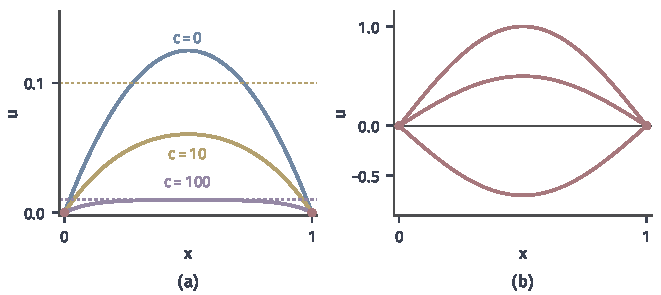
\includegraphics[width=112mm]{figures/06-differential-equations/02-partial-differential-equations/matplotlib/ellip-sign-failure/figure.pdf}
  \caption{零阶项的符号。(a)$-u''+cu=1$，零边界，$c=0,10,100$，点线是上界$u\leq1/c$（$c=0$时无此上界）。(b)$c=-\pi^2$时$u=A\sin(\pi x)$（红线，$A=1,\tfrac12,-\tfrac7{10}$）都满足齐次方程和零边界，最大值原理失效。}
  \label{fig:ellip-sign-failure}
\end{BookInlineFigure}

\paragraph{弱解的最大值原理}
定理~\ref{thm:ellip-general-max}要求$u\in C^2$。散度型方程的弱解有一个不需要二阶导数的版本，它把能量方法和最大值原理连在了一起。

设$u\in H^1(\Omega)$是式~\eqref{eq:ellip-divergence-form}的弱解，$f\leq0$，$\operatorname{Tr}u\leq M$。把$v=(u-M)^+$作为测试函数，这里用到$H^1$函数被截断后仍在$H^1$中，且$\nabla v=\nabla u\,\mathbf{1}_{\{u>M\}}$，$v$的迹为零，所以$v\in H^1_0(\Omega)$。

由弱形式和$f\leq0$，$v\geq0$，
\[
 \kappa_{\min}\lVert\nabla v\rVert_2^2\leq\int_\Omega\bm{A}\nabla v\cdot\nabla v\,\mathrm{d}\bm{x}=a(u,v)=\int_\Omega fv\,\mathrm{d}\bm{x}\leq0 .
\]
所以$\nabla v=0$，由Poincaré不等式$v=0$，即$u\leq M$几乎处处成立。这个证明不要求$\bm{A}$连续，也适用于前面那根两段材料的棒。

\paragraph{两种估计的对比}
能量估计与最大值估计回答不同的问题，见表~\ref{tab:ellip-energy-vs-max}。两者不能互相替代：弱解的能量估计不给出逐点的界，而最大值原理不给出梯度的积分界。

\begin{BookInlineTable}
  \centering
  \caption{能量估计与最大值估计的对比。}
  \label{tab:ellip-energy-vs-max}
  \begin{tabular}{lll}
    \toprule
    & 能量估计 & 最大值估计\\
    \midrule
    控制的量 & $\lVert\nabla u\rVert_2$（平方平均） & $\max\lvert u\rvert$（逐点）\\
    数据的度量 & $\lVert f\rVert_2$ & $\sup\lvert f\rvert$\\
    结构要求 & 强制性 & 符号（$c\geq0$）\\
    适用范围 & 方程组同样可用 & 只对标量方程\\
    \bottomrule
  \end{tabular}
\end{BookInlineTable}


\section{正则性}
\label{sec:ellip-regularity}

Lax--Milgram定理给出的弱解只在$H^1$中。它是否具有更好的性质，比如二阶导数平方可积、逐点连续，甚至光滑？这决定了弱解是否就是经典解，也决定了数值方法能达到多高的精度。答案取决于系数、源项和区域三者，而且内部和边界的情况不一样。

\paragraph{一维的情形}
在一维可以直接看到。$-u''=f$的弱解满足$u''=-f$，所以$f\in L^2$时$u\in H^2$，$f$连续时$u\in C^2$，一般地$f\in C^k$时$u\in C^{k+2}$。解比源项多两阶导数，这正是“两次积分”的效果。

图~\ref{fig:ellip-regularity-ladder}取跳跃的源项$f=\mathbf{1}_{(1/2,1)}$，零边界。解$u$的二阶导数就是$-f$，有跳跃，所以$u\in H^2$但$u\notin C^2$。$u'$连续但有折角，$u$是$C^1$的，已经看不出任何异常。

\begin{BookInlineFigure}
  \centering
  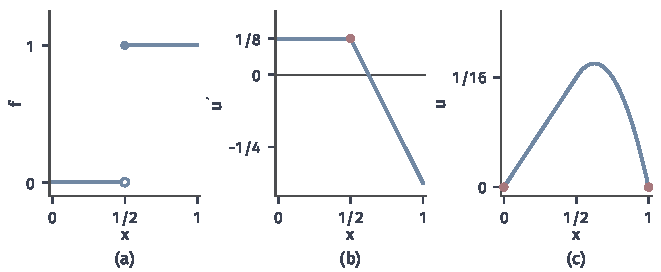
\includegraphics[width=112mm]{figures/06-differential-equations/02-partial-differential-equations/matplotlib/ellip-regularity-ladder/figure.pdf}
  \caption{解比源项多两阶光滑性。(a)源项$f$在$x=1/2$处跳跃。(b)$u'$连续，在红点处有折角。(c)$u$是$C^1$的，曲线在中点看不出异常。由式~\eqref{eq:ellip-interval-solution}，$x\leq1/2$时$u=x/8$，$x\geq1/2$时$u=1/16+(x-\tfrac12)/8-(x-\tfrac12)^2/2$。}
  \label{fig:ellip-regularity-ladder}
\end{BookInlineFigure}

这种增益来自源项，前提是系数足够好。图~\ref{fig:ellip-coefficient-jump}的两段材料中，$f=1$是光滑的，解在界面处却有折角，$u'$有跳跃，$u\notin H^2$。方程能保证的是通量$au'$在$H^1$中，而把$a$除掉后，$u'$的光滑性不会比$a$好。这说明系数必须有一定的光滑性才能得到$H^2$。

\paragraph{为什么Laplace算子能控制全部二阶导数}
多维的情形有一个疑问：方程只给出了$\Delta u$，即二阶导数的一个特定组合，它凭什么控制全部的二阶导数？对$v\in C_c^\infty(\mathbb{R}^{d})$，分部积分两次，
\[
 \int\partial_i\partial_jv\,\partial_i\partial_jv\,\mathrm{d}\bm{x}=\int\partial_i\partial_iv\,\partial_j\partial_jv\,\mathrm{d}\bm{x}.
\]
对$i,j$求和，得到恒等式
\begin{equation}
 \lVert\nabla^2v\rVert_2=\lVert\Delta v\rVert_2 .
 \label{eq:ellip-hessian-identity}
\end{equation}
Hessian的全部元素的平方和，积分后恰好等于$\Delta v$的平方的积分。这个恒等式是椭圆方程内部正则性的核心，其中分部积分需要$v$紧支撑，边界项才能消失。

\paragraph{内部正则性}
定理的形式是：系数Lipschitz，$f\in L^2$，则弱解在内部多一阶导数。我们对$\bm{A}=\bm{I}$完整证明。一般系数的证明思路相同，差商落在系数上会多出一些低阶项，用系数的Lipschitz常数控制，读者可查阅椭圆方程的专著。

\begin{theorem}[内部$H^2$正则性]
\label{thm:ellip-interior}
设$\Omega$是开集，$\bm{A}$一致椭圆且Lipschitz连续，$f\in L^2(\Omega)$，$u\in H^1(\Omega)$满足$a(u,v)=\int_\Omega fv$对所有$v\in C_c^\infty(\Omega)$成立。则对每个$\Omega'$，只要$\overline{\Omega'}$是$\Omega$的紧子集，就有$u\in H^2(\Omega')$，且存在依赖于$\Omega'$和$\bm{A}$的常数$C$，使
\begin{equation}
 \lVert\nabla^2u\rVert_{L^2(\Omega')}\leq C\bigl(\lVert f\rVert_2+\lVert\nabla u\rVert_2\bigr).
 \label{eq:ellip-interior}
\end{equation}
\end{theorem}

注意定理对$u$的边界行为没有任何要求，这是内部正则性的特点。证明的关键技巧是用差商代替导数，因为我们还不知道二阶导数存在，而差商总是存在的。

\begin{proof}[$\bm{A}=\bm{I}$时的证明]
固定方向$\bm{e}_k$，对小的$h\neq0$定义差商
\[
 D^h\phi(\bm{x})=\frac{\phi(\bm{x}+h\bm{e}_k)-\phi(\bm{x})}h .
\]
在下面用到的区域和$h$范围内，有三条性质。

第一，分部求和：若$\phi$或$\psi$紧支撑，$\int(D^h\phi)\psi=-\int\phi\,D^{-h}\psi$。第二，差商不超过导数：设$\phi\in H^1(\Omega)$，$\overline{\Omega''}$是$\Omega$的紧子集，$\lvert h\rvert$小于$\Omega''$到$\partial\Omega$的距离，则由微积分基本定理和Cauchy--Schwarz不等式，
\[
 \lVert D^h\phi\rVert_{L^2(\Omega'')}\leq\lVert\partial_k\phi\rVert_{L^2(\Omega)} .
\]

第三，若$\lVert D^h\phi\rVert_{L^2(\Omega')}$对所有小的$h$有上界$B$，则$\partial_k\phi\in L^2(\Omega')$，且范数不超过$B$。这是因为有界序列$D^{h_n}\phi$有弱收敛子列，把弱极限记为$\Gamma$，对紧支撑的光滑$\psi$有
\[
 \int\Gamma\psi\,\mathrm{d}\bm{x}=-\lim_{n\to\infty}\int\phi\,D^{-h_n}\psi\,\mathrm{d}\bm{x}=-\int\phi\,\partial_k\psi\,\mathrm{d}\bm{x},
\]
所以$\Gamma=\partial_k\phi$。

取$\Omega''$介于$\Omega'$与$\Omega$之间，取截断函数$\eta\in C_c^\infty(\Omega'')$，$0\leq\eta\leq1$，在$\Omega'$上$\eta=1$。记$w=D^hu$，把测试函数取成
\[
 v=-D^{-h}(\eta^2w)\in H^1_0(\Omega) .
\]

由第一条性质，左端变成
\[
 \begin{aligned}
 \int_\Omega\nabla u\cdot\nabla v\,\mathrm{d}\bm{x}&=\int_\Omega\nabla w\cdot\nabla(\eta^2w)\,\mathrm{d}\bm{x}\\
 &=\int_\Omega\eta^2\lVert\nabla w\rVert_2^2\,\mathrm{d}\bm{x}+2\int_\Omega\eta w\,\nabla\eta\cdot\nabla w\,\mathrm{d}\bm{x}.
 \end{aligned}
\]

记$X=\lVert\eta\nabla w\rVert_2$，$B=\lVert w\nabla\eta\rVert_2$。由第二条性质和$0\leq\eta\leq1$，
\[
 \lVert v\rVert_2\leq\lVert\nabla(\eta^2w)\rVert_2\leq X+2B .
\]
$w$的大小也由第二条性质控制，所以$B$不超过$\nabla\eta$的上界与$\lVert\nabla u\rVert_2$的乘积。

把弱形式代入，由Cauchy--Schwarz不等式，得到
\[
 X^2\leq\lVert f\rVert_2(X+2B)+2XB .
\]
用$ab\leq\tfrac14a^2+b^2$吸收含$X$的项，
\[
 \frac12X^2\leq2\lVert f\rVert_2^2+5B^2 .
\]

所以
\[
 \lVert\nabla D^hu\rVert_{L^2(\Omega')}\leq X\leq C\bigl(\lVert f\rVert_2+\lVert\nabla u\rVert_2\bigr),
\]
上界与$h$无关。第三条性质用于每个分量$\partial_ju$，就得到$\partial_k\partial_ju\in L^2(\Omega')$和式~\eqref{eq:ellip-interior}。
\end{proof}

这个结果可以反复使用。$\bm{A}=\bm{I}$时，若$f\in H^1$，$\partial_ku$是源项为$\partial_kf$的弱解，再用一次定理得到$u$在内部属于$H^3$。一般地，$\bm{A}\in C^{k+1}$且$f\in H^k$时，$u$在内部属于$H^{k+2}$。特别地，系数和$f$都光滑时，弱解在内部光滑，调和函数是$C^\infty$的。由Sobolev嵌入，$k>d/2$时$H^k$函数有连续代表，所以$d\leq3$时内部的$H^2$解已经是连续函数。

$L^2$型的增益是整两阶。逐点的情形略有不同，$f$连续不足以保证$u\in C^2$，需要$f$是Hölder连续的。对应的结论称为Schauder估计，证明需要用基本解的奇异积分细致估计，篇幅较长，读者可查阅椭圆方程的专著。其结论是：$\bm{A},f\in C^{0,\gamma}$时$u\in C^{2,\gamma}$在内部成立。

若$\bm{A}$只是有界可测，则没有$H^2$可言，但De Giorgi和Nash的定理仍然给出弱解在内部的Hölder连续性（$f\in L^q$，$q>d/2$），证明同样需要较长的迭代估计，读者可查阅相关专著。

\paragraph{边界正则性}
内部估计依靠截断函数把边界隔开，边界附近没有这个便利，边界的形状成为新的约束。典型的结论如下。

\begin{theorem}[整体$H^2$正则性]
\label{thm:ellip-boundary}
设$\Omega$是有界开集，边界$\partial\Omega$属于$C^{1,1}$，$\bm{A}$在$\overline\Omega$上Lipschitz连续且一致椭圆，$f\in L^2(\Omega)$，$u\in H^1_0(\Omega)$是Dirichlet问题的弱解。则$u\in H^2(\Omega)$，且存在只依赖于$\Omega,\bm{A}$的常数$C$，使
\begin{equation}
 \lVert u\rVert_{H^2(\Omega)}\leq C\lVert f\rVert_2 .
 \label{eq:ellip-boundary-regularity}
\end{equation}
\end{theorem}

证明要把边界局部拉直，篇幅较长，读者可查阅椭圆方程的专著。思路是：拉直后边界是一块平面，沿切向的差商不改变测试函数的零迹，所以内部的论证对切向导数仍然成立，得到除$\partial_{\bm{n}}^2u$之外的二阶导数的估计；剩下的那一个由方程解出，因为方程把它写成了其余二阶导数和$f$的组合。Neumann问题也有类似结论，需要边界数据有相应的光滑性。

$\Omega$是凸多边形且$\bm{A}=\bm{I}$时结论仍成立，并且对零边界的函数有$\lVert\nabla^2u\rVert_2\leq\lVert\Delta u\rVert_2$，证明需要分析边界项的符号，读者可查阅相关专著。但只要边界有向内凹进去的角，结论就失效。

\paragraph{角点}
图~\ref{fig:ellip-corner}的区域是L形，内角$\omega=3\pi/2$的顶点在原点。用极坐标$(r,\theta)$，$\theta\in(0,3\pi/2)$，函数
\begin{equation}
 u=r^{2/3}\sin\frac{2\theta}{3}
 \label{eq:ellip-corner}
\end{equation}
在区域内调和，因为它是复解析函数$z^{2/3}$的虚部，并且在顶点相邻的两条边$\theta=0$、$\theta=3\pi/2$上为零。

\begin{BookInlineFigure}
  \centering
  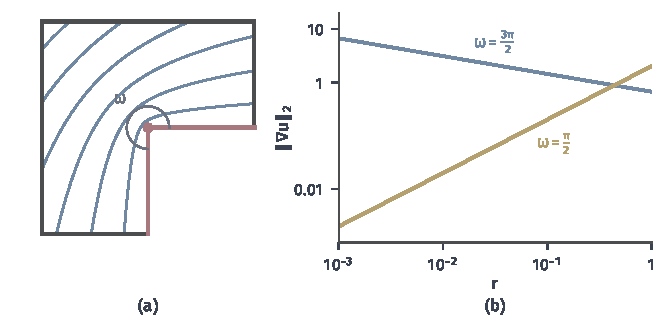
\includegraphics[width=112mm]{figures/06-differential-equations/02-partial-differential-equations/matplotlib/ellip-corner/figure.pdf}
  \caption{角点限制整体光滑性。(a)L形区域上$u=r^{2/3}\sin(2\theta/3)$的等值线，红色的两条边上$u=0$，它们在内角$\omega=3\pi/2$的顶点相交。(b)梯度大小随$r$的变化：$\omega=3\pi/2$时（蓝）$\frac23r^{-1/3}$在顶点爆炸，$\omega=\pi/2$的$r^2\sin2\theta$（黄）梯度$2r$在顶点趋于零。}
  \label{fig:ellip-corner}
\end{BookInlineFigure}

梯度的大小是$\frac23r^{-1/3}$，在顶点处趋于无穷，但其平方可积：
\[
 \int_0^1r^{-2/3}\,r\,\mathrm{d}r<\infty .
\]
所以$u\in H^1$，它是合法的弱解。二阶导数的大小是$r^{-4/3}$量级，平方的积分
\[
 \int_0^1r^{-8/3}\,r\,\mathrm{d}r
\]
发散，所以$u\notin H^2$。再取一个在顶点附近恒为$1$、支撑很小的光滑截断函数$\eta$，令$\tilde u=\eta u$。由乘积法则和$\Delta u=0$，
\[
 -\Delta\tilde u=-2\nabla\eta\cdot\nabla u-u\,\Delta\eta ,
\]
它只在$\eta$不是常数的地方非零，那里$u$光滑。所以$\tilde u$是光滑源项、全零边界值的问题的弱解，在顶点附近却与$u$相同，不属于$H^2$。

一般地，内角$\omega$对应的奇性是$r^{\pi/\omega}$。二阶导数的量级是$r^{\pi/\omega-2}$，平方可积当且仅当$\pi/\omega>1$，即$\omega<\pi$。内角超过$\pi$时奇性无法避免，这不是系数或数据的问题，而是几何本身的限制。

边界条件类型的切换也会产生奇性，哪怕边界本身是光滑的。在上半平面取$u=r^{1/2}\sin(\theta/2)$，它在正半轴$\theta=0$上满足$u=0$，在负半轴$\theta=\pi$上满足$\partial_\theta u=0$。切换点处的梯度量级是$r^{-1/2}$，同样不在$H^2$中。

把各种因素放在一起，可以这样理解：弱解的存在由能量和强制性决定，对光滑性没有要求；更高的光滑性是额外的收获，需要系数、源项和边界几何都配合，其中任何一个粗糙都会限制最终的结果。第~\ref{chap:pde-numerical-methods}章的有限元收敛阶，正是由这里的正则性决定的。


\section{本章小结}
\label{sec:ellip-summary}

开篇的问题是：平衡场的每一点由什么决定？本章的回答是，由整个区域内的源项和整条边界上的数据共同决定，这种全局依赖体现在解的每一种表示之中。

\paragraph{解的结构}
区间上的两次积分展示了最基本的结构：边界贡献和源项贡献线性相加，积分常数由边界条件确定。Green函数把源项的贡献写成点源响应的叠加，$G=\Phi-h$把点源的奇性和边界的修正分开；差分矩阵的逆是它的离散版本。谱展开把算子对角化，$u_k=f_k/\lambda_k$说明解比数据多两阶的光滑性，零特征值则要求先处理核空间。这些公式依赖几何或边界的特殊结构，适用范围有限，也都要求足够的光滑性。

\paragraph{弱理论}
弱形式把一阶导数分给测试函数，让系数跳变和粗糙的源都能进入问题。本质边界条件写进空间，自然边界条件写进积分。Lax--Milgram定理把适定性归结为有界、强制和右端连续三个条件，其证明由Riesz表示和强制性下界完成。三类边界条件的区别，在于怎样处理常数方向，见表~\ref{tab:ellip-summary}。

\begin{BookInlineTable}
  \centering
  \caption{三类边界条件的适定性（$\Omega$有界连通，$\bm{A}$一致椭圆）。}
  \label{tab:ellip-summary}
  \begin{tabular}{lll}
    \toprule
    条件 & 如何排除常数 & 可解性与唯一性\\
    \midrule
    Dirichlet & 零迹与Poincaré不等式 & 任意数据，唯一\\
    Neumann & 零均值子空间 & 需相容条件，差常数\\
    Robin & 边界代价，$\int\beta>0$ & 任意数据，唯一\\
    \bottomrule
  \end{tabular}
\end{BookInlineTable}

\paragraph{三种进一步的结构}
对称问题的弱解是能量的唯一极小点，能量差恰好是误差在能量范数下的平方；非对称问题仍可用Lax--Milgram定理，但没有这种极小刻画。最大值原理依靠符号结构控制逐点的大小，$c\geq0$是必要的结构条件。正则性在内部由系数和源项决定，整体还受边界几何和边界条件切换点的限制。

\paragraph{结论的适用范围}
能量方法和Lax--Milgram定理给出弱解的存在和唯一，对边界和系数的要求很低。最大值原理要求符号条件，经典形式要求解是$C^2$的，弱形式的版本用截断测试函数绕过了这一点。更高的光滑性要求系数、源项和边界同时配合。所有这些结论都是关于平衡场的，没有时间的参与。

第~\ref{chap:diffusion-equations}章在同样的空间和边界模式上引入时间，第~\ref{chap:pde-numerical-methods}章把这里的弱形式在有限维子空间上离散，得到有限元方法。

